\documentclass[conference,compsoc]{IEEEtran}
% Submission format: IEEEtran, conference + compsoc, US letter, no margin or font changes.
\usepackage{amsmath,amssymb,amsthm}
\usepackage{graphicx}
\usepackage{booktabs}
\usepackage{array}
\usepackage{cite}
\usepackage{xurl}
\usepackage{xcolor}
\usepackage[hidelinks]{hyperref}
\newcommand{\artifactlink}[1]{\texorpdfstring{\href{https://github.com/submissionrepo/buying-time-artifact}{\textcolor{blue}{#1}}}{#1}}

% Generated by make_numbers.py; do not edit by hand.
\newcommand{\nRecords}{69}
\newcommand{\nExcluded}{12}
\newcommand{\nEvents}{57}
\newcommand{\valueEventsB}{3.7}
\newcommand{\valueEventsM}{3,711}
\newcommand{\eventsFirstYear}{2021}
\newcommand{\eventsLastYear}{2026}
\newcommand{\medOutflowMin}{8}
\newcommand{\medOutflowWords}{eight}
\newcommand{\medRespH}{3}
\newcommand{\medRespM}{42}
\newcommand{\nTimedEvents}{48}
\newcommand{\nUntimedEvents}{9}
\newcommand{\shareTenMinPct}{68}
\newcommand{\nShareTenMin}{38}
\newcommand{\nPaused}{19}
\newcommand{\nPausedAfterLast}{17}
\newcommand{\nRespAck}{30}
\newcommand{\nRespPause}{18}
\newcommand{\lateOneEventsPct}{83}
\newcommand{\lateOneValuePct}{91}
\newcommand{\lateSixEventsPct}{35}
\newcommand{\lateSixValuePct}{23}
\newcommand{\lateDayEventsPct}{10}
\newcommand{\lateDayValuePct}{19}
\newcommand{\lateTwoDaysEventsPct}{8}
\newcommand{\lateTwoDaysValuePct}{19}
\newcommand{\classVPct}{32}
\newcommand{\nClassV}{21}
\newcommand{\classDPct}{57}
\newcommand{\nClassD}{25}
\newcommand{\classSPct}{11}
\newcommand{\nClassS}{6}
\newcommand{\classOPct}{0.3}
\newcommand{\nClassO}{5}
\newcommand{\sideEscrowPct}{63}
\newcommand{\sideMintPct}{19}
\newcommand{\sideBothPct}{18}
\newcommand{\valueTimedB}{3.7}
\newcommand{\valueTimedM}{3,672}
\newcommand{\valueUntimedM}{39}
\newcommand{\rampOneMPct}{87.2}
\newcommand{\rampPointOneMPct}{97.3}
\newcommand{\rampTenMPct}{59.3}
\newcommand{\rampThirtyMPct}{35.0}
\newcommand{\cliffDayPct}{80.7}
\newcommand{\cliffOneHPct}{8.9}
\newcommand{\cliffSixHPct}{76.4}
\newcommand{\cliffThreeDPct}{84.8}
\newcommand{\freezeOneMPct}{97.4}
\newcommand{\freezeTenMPct}{90.1}
\newcommand{\freezeHundredMPct}{48.6}
\newcommand{\verifierMaxPct}{27.0}
\newcommand{\verifierCeilNoTopThreePct}{51.2}
\newcommand{\verifierRampThirtyMPct}{10.5}
\newcommand{\valueClassSTimedM}{406}
\newcommand{\matchSmallTwelvePct}{85.4}
\newcommand{\matchFullTwelvePct}{75.3}
\newcommand{\matchSmallTwentyFourPct}{58.6}
\newcommand{\matchFullTwentyFourPct}{32.1}
\newcommand{\matchEnvFourHM}{10.7}
\newcommand{\matchEnvFourHTwentyFourM}{46.0}
\newcommand{\robRampTimesTwoPct}{80.3}
\newcommand{\robRampPlusSixPct}{83.3}
\newcommand{\robRampPausesPct}{89.7}
\newcommand{\robPausesN}{18}
\newcommand{\robRampEventPct}{32}
\newcommand{\robRampNoLargestPct}{85.0}
\newcommand{\robLargestSharePct}{17}
\newcommand{\robCliffEventPct}{79}
\newcommand{\robMatchEventPct}{25}
\newcommand{\robMatchFullEventPct}{19}
\newcommand{\matchEnvFourHFullM}{30.9}
\newcommand{\matchEnvFourHFullTwentyFourM}{120}
\newcommand{\robVerifierMaxPct}{36.7}
\newcommand{\robVerifierTopThreePct}{48.5}
\newcommand{\stakeFlowMedianM}{30.9}
\newcommand{\stakeFlowMeanM}{49.8}
\newcommand{\stakeFlowReviewMeanM}{29.2}
\newcommand{\oneBucketWormThreeH}{1.14}
\newcommand{\oneBucketWormSixH}{1.07}
\newcommand{\oneBucketWormDay}{1.00}
\newcommand{\oneBucketCcipOneMed}{1.13}
\newcommand{\oneBucketCcipOneMax}{2.38}
\newcommand{\oneBucketCcipOneMedPct}{13}
\newcommand{\oneBucketCcipSixMed}{1.05}
\newcommand{\oneBucketCcipSixMax}{1.57}
\newcommand{\oneBucketCcipSixMedPct}{5}
\newcommand{\plRampSepPct}{87.2}
\newcommand{\plRampGovPct}{80.6}
\newcommand{\plRampPessPct}{75.8}
\newcommand{\plRampVerPct}{25.5}
\newcommand{\plRampContractPct}{82.8}
\newcommand{\rtRampTwoPct}{80.3}
\newcommand{\rtRampFivePct}{68.4}
\newcommand{\rtRampTenPct}{62.8}
\newcommand{\rtRampOutflowPct}{62.8}
\newcommand{\rtRampNoPausePct}{80.6}
\newcommand{\rtRampAlertPct}{87.9}
\newcommand{\rtRampAlarmPct}{97.2}
\newcommand{\rtRampAlarmHourPct}{96.1}
\newcommand{\rtRampAllPct}{86.3}
\newcommand{\wtRampEventPct}{32}
\newcommand{\wtRampNetPct}{79.2}
\newcommand{\plHoldSepPct}{80.7}
\newcommand{\plHoldGovPct}{73.7}
\newcommand{\plHoldPessPct}{68.5}
\newcommand{\plHoldVerPct}{26.7}
\newcommand{\plHoldContractPct}{76.9}
\newcommand{\rtHoldTwoPct}{79.8}
\newcommand{\rtHoldFivePct}{71.8}
\newcommand{\rtHoldTenPct}{25.4}
\newcommand{\rtHoldOutflowPct}{64.9}
\newcommand{\rtHoldNoPausePct}{73.5}
\newcommand{\rtHoldAlertPct}{80.7}
\newcommand{\rtHoldAlarmPct}{99.7}
\newcommand{\rtHoldAlarmHourPct}{99.7}
\newcommand{\rtHoldAllPct}{79.9}
\newcommand{\wtHoldEventPct}{79}
\newcommand{\wtHoldNetPct}{67.6}
\newcommand{\plMatchSepPct}{75.3}
\newcommand{\plMatchGovPct}{71.1}
\newcommand{\plMatchPessPct}{68.2}
\newcommand{\plMatchVerPct}{20.7}
\newcommand{\plMatchContractPct}{72.0}
\newcommand{\rtMatchTwoPct}{71.7}
\newcommand{\rtMatchFivePct}{63.9}
\newcommand{\rtMatchTenPct}{56.9}
\newcommand{\rtMatchOutflowPct}{53.5}
\newcommand{\rtMatchNoPausePct}{71.1}
\newcommand{\rtMatchAlertPct}{75.5}
\newcommand{\rtMatchAlarmPct}{79.1}
\newcommand{\rtMatchAlarmHourPct}{79.1}
\newcommand{\rtMatchAllPct}{74.5}
\newcommand{\wtMatchEventPct}{19}
\newcommand{\wtMatchNetPct}{67.0}
\newcommand{\vKeysCtrlN}{12}
\newcommand{\vN}{21}
\newcommand{\vKeysCtrlValuePct}{10.9}
\newcommand{\dFlawReachN}{2}
\newcommand{\dN}{25}
\newcommand{\noPauseValuePct}{11}
\newcommand{\outflowDetectedN}{20}
\newcommand{\outflowDetectedValuePct}{31}
\newcommand{\breakevenRamp}{22.5}
\newcommand{\breakevenMatch}{23.75}
\newcommand{\meanRespH}{50}
\newcommand{\bestOneBDStarH}{13}
\newcommand{\bestOneBGainPct}{2}
\newcommand{\bestTwoBDStarH}{50}
\newcommand{\bestTwoBGainPct}{13}
\newcommand{\kBucketsHullPct}{6}
\newcommand{\kBucketsEnvPct}{19}
\newcommand{\detThirdParty}{21}
\newcommand{\detOperator}{10}
\newcommand{\detUnknown}{23}
\newcommand{\detShortfall}{2}
\newcommand{\pauseIndependent}{39}
\newcommand{\pauseNone}{9}
\newcommand{\pauseControlled}{4}
\newcommand{\pauseUnknown}{5}
\newcommand{\classAgree}{53}
\newcommand{\nRecovered}{20}
\newcommand{\recoveredM}{1,744}
\newcommand{\recoveredPct}{47}
\newcommand{\nSingleChain}{36}
\newcommand{\nBorderline}{37}
\newcommand{\ccipInTodayDelayedPct}{19.3}
\newcommand{\ccipInTodayMeanDelayH}{0.53}
\newcommand{\ccipInTodayWaitPFifty}{1.3}
\newcommand{\ccipRevDelayedPct}{0.8}
\newcommand{\ccipRevMeanDelayH}{0.014}
\newcommand{\ccipRevPerMonth}{2.4}
\newcommand{\ccipRevValuePct}{24}
\newcommand{\ccipRevCapOne}{0.62}
\newcommand{\ccipRevCapSix}{0.52}
\newcommand{\ccipRevBreakevenH}{2.2}
\newcommand{\ccipRevAtOneH}{0.25}
\newcommand{\ccipRevVariants}{six}
\newcommand{\ccipRevLowerBoth}{Five}
\newcommand{\ccipRevBreakevenMinH}{1.6}
\newcommand{\ccipRevBreakevenMaxH}{2.5}
\newcommand{\roninReviewN}{five}
\newcommand{\roninReleasesAll}{74,282}
\newcommand{\roninReviewMinH}{15}
\newcommand{\roninReviewMedH}{62}
\newcommand{\roninReviewMaxD}{7.8}
\newcommand{\ccipEthLagPOneMin}{14}
\newcommand{\ccipEthLagMedMin}{17}
\newcommand{\ccipNoRevDelayedPct}{8.3}
\newcommand{\ccipNoRevMeanDelayH}{10.8}
\newcommand{\ccipNoRevWaitPFifty}{27}
\newcommand{\ccipNoRevCapSix}{0.60}
\newcommand{\ccipLanesDisabledHalf}{5}
\newcommand{\ccipInLanes}{16}
\newcommand{\ccipEntries}{2,992}
\newcommand{\ccipEnabled}{2,021}
\newcommand{\ccipActive}{1,682}
\newcommand{\ccipNearZero}{331}
\newcommand{\ccipRefillOneH}{450}
\newcommand{\ccipRefillDay}{586}
\newcommand{\ccipMedRefillH}{6.0}
\newcommand{\ccipMedCapK}{623}
\newcommand{\ccipCapQOneK}{108}
\newcommand{\ccipCapQThreeM}{2.55}
\newcommand{\ccipMedRateK}{108}
\newcommand{\ccipTokens}{168}
\newcommand{\ccipSelLanes}{18}
\newcommand{\ccipSelSharePct}{53.9}
\newcommand{\ccipFitLanes}{18}
\newcommand{\ccipFitLanesBucket}{17}
\newcommand{\ccipLooseOne}{7}
\newcommand{\ccipTightOne}{10}
\newcommand{\ccipRatioMinOne}{0.17}
\newcommand{\ccipRatioMaxOne}{7.69}
\newcommand{\ccipInSampleDelayedOne}{0}
\newcommand{\ccipLooseSix}{9}
\newcommand{\ccipTightSix}{8}
\newcommand{\ccipRatioMinSix}{0.31}
\newcommand{\ccipRatioMaxSix}{13.38}
\newcommand{\ccipInSampleDelayedSix}{0}
\newcommand{\ccipOosLanes}{18}
\newcommand{\ccipOosZero}{8}
\newcommand{\ccipOosMaxPct}{88}
\newcommand{\ccipOosOverHalf}{3}
\newcommand{\ccipLanes}{17}
\newcommand{\ccipLanesBucket}{16}
\newcommand{\ccipCurrentDelayedPct}{21.2}
\newcommand{\ccipSixDelayedPct}{8.3}
\newcommand{\ccipSixRatio}{0.66}
\newcommand{\ccipSixTwoDelayedPct}{4.5}
\newcommand{\ccipSixTwoRatio}{0.88}
\newcommand{\ccipOneTwoDelayedPct}{5.8}
\newcommand{\ccipOneTwoRatio}{1.71}
\newcommand{\poolLow}{2.6}
\newcommand{\poolHigh}{2.7}
\newcommand{\poolRatioLowPct}{37}
\newcommand{\poolRatioHighPct}{39}
\newcommand{\wormChains}{9}
\newcommand{\wormChainsWords}{nine}
\newcommand{\wormEnvOneHFullM}{30.0}
\newcommand{\wormEnvOneHSmallM}{8.7}
\newcommand{\wormEnvRatio}{3.4}
\newcommand{\wormEnvDayFullM}{42.8}
\newcommand{\wormEnvDaySmallM}{29.6}
\newcommand{\wormBigN}{397}
\newcommand{\wormBigValuePct}{8.2}
\newcommand{\wormBigTwelveN}{53}
\newcommand{\wormBigTwelveValuePct}{5.8}
\newcommand{\govSuiHours}{415}
\newcommand{\govSuiPct}{2.4}
\newcommand{\govEthHours}{13}
\newcommand{\govOtherMaxHours}{75}
\newcommand{\govChains}{9}
\newcommand{\stakeMaxRatio}{0.16}
\newcommand{\stakeLargeMinM}{16}
\newcommand{\stakeLargeMaxM}{529}
\newcommand{\stakeLargeN}{three}
\newcommand{\stakeLargeCoverWords}{Two}
\newcommand{\stakeLargeCoverLow}{two}
\newcommand{\stakeLinkM}{529}
\newcommand{\stakePolygonM}{342}
\newcommand{\stakeAxelarM}{16}
\newcommand{\stakeSlashableMaxM}{1.3}
\newcommand{\stakeEmptyVaults}{4}
\newcommand{\stakeEmptyVaultsWords}{four}
\newcommand{\stakeBlock}{26,201,369}
\newcommand{\stakeAxelarHeight}{36,297,293}
\newcommand{\nRules}{22}
\newcommand{\nRulesBounded}{4}
\newcommand{\nRulesBoundedWords}{four}
\newcommand{\nRulesBoundedControlled}{3}
\newcommand{\nRulesBoundedControlledWords}{three}
\newcommand{\nRulesVerifierSide}{4}
\newcommand{\nRulesVerifierSideWords}{four}
\newcommand{\nRulesAutoRelease}{7}
\newcommand{\nRulesAutoReleaseWords}{seven}
\newcommand{\nRulesNet}{6}
\newcommand{\nRulesNetWords}{six}
\newcommand{\nRulesNetSameToken}{4}
\newcommand{\nRulesNetSameTokenWords}{four}
\newcommand{\gasPlain}{38,135}
\newcommand{\gasWindow}{71,473}
\newcommand{\gasWindowExtra}{33,338}
\newcommand{\gasQueue}{100,716}
\newcommand{\gasExecute}{62,824}
\newcommand{\gasExecuteMint}{62,404}
\newcommand{\gasLimiter}{163,540}
\newcommand{\gasLimiterExtra}{125,405}
\newcommand{\gasCancel}{30,032}
\newcommand{\gasPause}{29,662}
\newcommand{\gasHashSaving}{44,200}
\newcommand{\nTests}{48}
\newcommand{\invRuns}{256}
\newcommand{\invDepth}{100}
\newcommand{\nRulesReleaseOutside}{13}
\newcommand{\nRulesReleaseOutsideWords}{thirteen}
\newcommand{\nRulesReleasePartlyWords}{three}
\newcommand{\nRulesSendOnlyWords}{one}
\newcommand{\nRulesNoPauseWords}{Five}
\newcommand{\ccipGriefDayM}{3.2}
\newcommand{\ccipMisLanes}{17}
\newcommand{\ccipInLooseOne}{7}
\newcommand{\ccipInTightOne}{10}
\newcommand{\ccipInRatioMinOne}{0.17}
\newcommand{\ccipInRatioMaxOne}{8.09}
\newcommand{\ccipInLooseSix}{9}
\newcommand{\ccipInTightSix}{8}
\newcommand{\ccipInRatioMinSix}{0.34}
\newcommand{\ccipInRatioMaxSix}{13.94}
\newcommand{\ccipInEnabled}{1,986}
\newcommand{\ccipInOutSharePct}{98}
\newcommand{\ccipNoRefill}{8}
\newcommand{\classKappa}{0.92}
\newcommand{\nSecondDisagreeWords}{three}
\newcommand{\classSExactPct}{11.1}
\newcommand{\classSRecodedPct}{11.1}
\newcommand{\ceilHighPct}{27.4}
\newcommand{\ceilLowPct}{18.2}
\newcommand{\verifierVisiblePct}{27}
\newcommand{\nRedeemedLegs}{three}
\newcommand{\nVerifierChecksWords}{five}
\newcommand{\nSPossible}{5}
\newcommand{\nSDoubt}{2}
\newcommand{\nValidation}{13}
\newcommand{\nValidationWords}{thirteen}
\newcommand{\valTaikoQuota}{1,000}
\newcommand{\valTaikoUsed}{999}
\newcommand{\valRoninEthLock}{4,000}
\newcommand{\valRoninEthDaily}{4,500}
\newcommand{\valRoninEthUsed}{103}
\newcommand{\valRoninUsdcLockM}{2}
\newcommand{\valRoninUsdcDailyM}{2.5}
\newcommand{\valRoninUsdcUsed}{16,200}
\newcommand{\valTaikoRate}{41.7}
\newcommand{\valTaikoRead}{128.22}
\newcommand{\valTaikoBound}{297}
\newcommand{\valTaikoOut}{278}
\newcommand{\valTaikoPct}{94}
\newcommand{\valTaikoMaxPct}{99}
\newcommand{\valRoninEthBound}{4,397}
\newcommand{\valRoninEthOut}{3,996}
\newcommand{\valRoninEthPct}{91}
\newcommand{\valRoninUsdcBoundM}{2.48}
\newcommand{\valRoninUsdcOutM}{2.00}
\newcommand{\valRoninUsdcPct}{80}
\newcommand{\respBothN}{18}
\newcommand{\respPauseFirstN}{16}
\newcommand{\respAckAfterPauseH}{2.2}
\newcommand{\respPauseOnchainN}{13}
\newcommand{\respWeekendMedH}{3.5}
\newcommand{\respWeekdayMedH}{3.7}
\newcommand{\respWeekendP}{0.75}
\newcommand{\respHourP}{0.40}
\newcommand{\respIndepMedH}{3.1}
\newcommand{\respIndepN}{33}
\newcommand{\respEarlyMedH}{3.1}
\newcommand{\respEarlyN}{19}
\newcommand{\respLateMedH}{5.0}
\newcommand{\respLateN}{29}
\newcommand{\pbN}{20}
\newcommand{\pbNAllWords}{twenty}
\newcommand{\pbNWords}{sixteen}
\newcommand{\pbValueSharePct}{89}
\newcommand{\pbValueB}{3.3}
\newcommand{\pbFirstHistoryDays}{40}
\newcommand{\pbSelectionText}{every failure with a recorded response of at least \$20 million except Mixin, whose custody sat in hot wallets on many chains that we could not enumerate, and seven smaller ones whose release point we could read.}
\newcommand{\pbApartText}{four more are shown apart: the 2024 Ronin failure met a deployed limit (Section~\ref{sec:validation}), and Anyswap's routers, QBridge and the AFX bridge went into service 40, 59 and 71 days before their failures, too late for the fit below.}
\newcommand{\pbFloorPct}{71.4}
\newcommand{\pbFloorEventPct}{78}
\newcommand{\pbFloorLoPct}{49}
\newcommand{\pbFloorHiPct}{90}
\newcommand{\pbFloorNetPct}{57}
\newcommand{\pbLargestLossShare}{57}
\newcommand{\pbLargestLossDays}{6}
\newcommand{\pbLargestLegitDayM}{24}
\newcommand{\pbOthersN}{fifteen}
\newcommand{\pbOthersFloorPct}{85.4}
\newcommand{\pbBucketPct}{72.2}
\newcommand{\pbBucketEventPct}{76}
\newcommand{\pbBucketGovPct}{69.2}
\newcommand{\pbBucketFivePct}{67.2}
\newcommand{\pbBucketOutflowPct}{61.0}
\newcommand{\pbBucketDelayedPct}{17}
\newcommand{\pbBucketDelayedTwoPct}{48}
\newcommand{\pbBucketDelayedMaxPct}{98}
\newcommand{\pbBucketWaitMedH}{14}
\newcommand{\pbBucketHoursPerDollar}{4.7}
\newcommand{\pbBucketHoursPerDollarTwo}{41}
\newcommand{\pbReviewPct}{77.7}
\newcommand{\pbReviewEventPct}{82}
\newcommand{\pbReviewLoPct}{53}
\newcommand{\pbReviewHiPct}{96}
\newcommand{\pbReviewGovPct}{73.4}
\newcommand{\pbReviewOutflowPct}{65.8}
\newcommand{\pbReviewFivePct}{69.9}
\newcommand{\pbReviewDelayedPct}{2.4}
\newcommand{\pbReviewDelayedTwoPct}{1.0}
\newcommand{\pbReviewSharePct}{38}
\newcommand{\pbReviewShareTwoPct}{48}
\newcommand{\pbReviewTotalPct}{40}
\newcommand{\pbReviewTotalTwoPct}{49}
\newcommand{\pbReviewPerMonth}{14}
\newcommand{\pbReviewPerMonthTwo}{15}
\newcommand{\pbReviewWaitOneH}{0.4}
\newcommand{\pbReviewWaitOneHTwo}{0.5}
\newcommand{\pbReviewWaitSixH}{2.3}
\newcommand{\pbReviewWaitSixHTwo}{3.0}
\newcommand{\pbReviewWaitDayH}{9.1}
\newcommand{\pbReviewWaitDayHTwo}{11.7}
\newcommand{\pbReviewWaitOneMin}{26}
\newcommand{\pbTestTransfers}{115,811}
\newcommand{\pbTestTransfersTwo}{141,544}
\newcommand{\pbReviewAlarmHourPct}{94.5}
\newcommand{\pbReviewAlarmHourEventPct}{92}
\newcommand{\pbReviewAlarmHourLoPct}{92}
\newcommand{\pbReviewAlarmHourHiPct}{97}
\newcommand{\pbBucketAlarmHourPct}{73.0}
\newcommand{\pbFloorAlarmHourPct}{76.9}
\newcommand{\pbAlarmOnlyHourPct}{14}
\newcommand{\pbReviewAlarmTenPct}{95.4}
\newcommand{\pbReviewAlarmTenEventPct}{93}
\newcommand{\pbReviewAlarmTenLoPct}{93}
\newcommand{\pbReviewAlarmTenHiPct}{97}
\newcommand{\pbBucketAlarmTenPct}{73.4}
\newcommand{\pbFloorAlarmTenPct}{78.5}
\newcommand{\pbAlarmOnlyTenPct}{32}
\newcommand{\pbHundredPct}{85.1}
\newcommand{\pbHundredEventPct}{85}
\newcommand{\pbHundredSharePct}{66}
\newcommand{\pbHundredPerMonth}{92}
\newcommand{\pbHundredAlarmHourPct}{97.0}
\newcommand{\pbVarFloorPct}{78.9}
\newcommand{\pbVarReviewPct}{77.7}
\newcommand{\pbVarDroppedN}{three}
\newcommand{\pbPolyUnpricedPct}{43}
\newcommand{\pbPolyTwoUnpricedPct}{31}
\newcommand{\pbWinReviewPct}{77 to 78}
\newcommand{\pbBucketOnePct}{72.7}
\newcommand{\pbBucketOneDelayedPct}{16}
\newcommand{\pbBucketDayPct}{69.5}
\newcommand{\pbBucketDayDelayedPct}{18}
\newcommand{\pbBucketFiftyPct}{67.7}
\newcommand{\pbBucketFiftyDelayedPct}{20}
\newcommand{\pbGateMin}{10}
\newcommand{\pbFloorPctR}{71}
\newcommand{\pbBucketPctR}{72}
\newcommand{\pbReviewPctR}{78}
\newcommand{\pbGateWorksPctR}{100}
\newcommand{\pbReviewSparePct}{99.8}
\newcommand{\pbGateHoursPerDollar}{0.17}
\newcommand{\pbGateWorksPct}{100.0}
\newcommand{\pbGateFailsPct}{72.2}
\newcommand{\pbGateWorksMatchPct}{99.9}
\newcommand{\pbGateAloneFailsPct}{0}
\newcommand{\pbGateAloneWorksPct}{100}
\newcommand{\checkSeesPct}{99.7}
\newcommand{\checkMatchSeesPct}{89}
\newcommand{\checkKeysHeldVPct}{8}
\newcommand{\pbGateBuiltPct}{96}
\newcommand{\pbReviewCheckFailsPct}{8}
\newcommand{\pbReviewAlarmCheckFailsPct}{8}
\newcommand{\pbLoosePct}{63.9}
\newcommand{\pbLooseGateWorksPct}{100.0}
\newcommand{\pbLooseDelayedPct}{7}
\newcommand{\pbLooseDelayedTwoPct}{35}
\newcommand{\pbLooseHoursPerDollar}{1.4}
\newcommand{\pbLooseHoursPerDollarTwo}{9.7}
\newcommand{\pbBucketCountPct}{0.8}
\newcommand{\pbBucketCountTwoPct}{12.7}
\newcommand{\pbReviewCountPct}{0.4}
\newcommand{\pbReviewCountTwoPct}{0.3}
\newcommand{\pbLooseCountPct}{0.1}
\newcommand{\pbLooseCountTwoPct}{2.8}
\newcommand{\pbBucketWaitNinetyNineTwoH}{219}
\newcommand{\pbReviewPerMonthMed}{1}
\newcommand{\pbReviewPerMonthMax}{148}
\newcommand{\pbBucketKeysHeldPct}{69.2}
\newcommand{\pbReviewKeysHeldPct}{74.5}
\newcommand{\pbPauseFirstN}{ten}
\newcommand{\pbPauseFirstFloorPct}{65}
\newcommand{\pbPauseFirstBucketPct}{67}
\newcommand{\pbPauseFirstReviewPct}{71}
\newcommand{\pbBucketNetPct}{57}
\newcommand{\pbReviewNetPct}{63}
\newcommand{\pbGateWorksNetPct}{100}
\newcommand{\pbFloorLooLoPct}{66}
\newcommand{\pbFloorLooHiPct}{85}
\newcommand{\pbReviewLooLoPct}{73}
\newcommand{\pbReviewLooHiPct}{93}
\newcommand{\pbBucketLoPct}{49}
\newcommand{\pbBucketHiPct}{90}
\newcommand{\pbGateWorksLoPct}{100}
\newcommand{\pbRoninEnvM}{855}
\newcommand{\pbRoninOutsizedM}{722}
\newcommand{\pbRoninEnvTrimM}{342}
\newcommand{\pbRoninFloorTrimPct}{37}
\newcommand{\pbRoninTakenM}{540}
\newcommand{\dbLowerPct}{8}
\newcommand{\dbLowerTwoPct}{23}
\newcommand{\coverEntries}{92}
\newcommand{\coverMatched}{43}
\newcommand{\coverLeftOut}{9}
\newcommand{\coverSmall}{32}
\newcommand{\coverNotBridge}{seven}
\newcommand{\coverAfter}{33}
\newcommand{\fpPausedTimePct}{1.8}
\newcommand{\fpWaitPerDollar}{0.009}
\newcommand{\gasPriceGwei}{0.20}
\newcommand{\gasPriceNinetyGwei}{0.61}
\newcommand{\ethUsd}{2,441}
\newcommand{\gasExtraUsd}{0.06}
\newcommand{\gasExtraNinetyUsd}{0.19}
\newcommand{\gasExtraThirtyUsd}{9}
\newcommand{\gasTunedOne}{79,161}
\newcommand{\gasTunedFour}{95,981}
\newcommand{\gasTunedPerBucket}{5,606}
\newcommand{\gasTunedTotal}{207,384}
\newcommand{\gasTunedExtra}{169,249}
\newcommand{\gasTunedExtraUsd}{0.08}
\newcommand{\nTestsTuned}{12}
\newcommand{\nFuzzRuns}{1,000}
\newcommand{\blindN}{57}
\newcommand{\blindAgree}{55}
\newcommand{\blindKappa}{0.95}
\newcommand{\blindDisValuePct}{0.4}
\newcommand{\blindVerifierPct}{27}
\newcommand{\blindPauseAgree}{54}
\newcommand{\blindPauseN}{57}
\newcommand{\keysHeldPct}{17}
\newcommand{\keysHeldN}{8}
\newcommand{\tbForgedN}{12}
\newcommand{\tbForgedDetectMaxS}{12}
\newcommand{\tbForgedPauseMaxS}{12}
\newcommand{\tbForgedRecordReleasedM}{2.9}
\newcommand{\tbForgedPoints}{ten}
\newcommand{\tbReleasesOrbit}{4,152}
\newcommand{\tbReleasesNomad}{14,532}
\newcommand{\tbLegitRequests}{56,052}
\newcommand{\tbNomadDelayedPct}{14}
\newcommand{\tbBurstOrbitM}{2.6}
\newcommand{\tbBurstNomadM}{13.1}
\newcommand{\tbFalseAlarms}{0}
\newcommand{\tbEpisodes}{636}
\newcommand{\tbRuns}{four}
\newcommand{\tbPauseMaxS}{60}
\newcommand{\tbHoldReleased}{0}
\newcommand{\tbFinalityGapMinM}{10}
\newcommand{\tbFinalityGapMaxM}{12}
\newcommand{\tbReorgTargets}{119}
\newcommand{\tbReorgOnceMax}{19}
\newcommand{\tbReorgRecheckMaxS}{48}
\newcommand{\tbRtPauseMinS}{2}
\newcommand{\tbRtPauseMaxS}{60}
\newcommand{\tbRtEpisodes}{36}
\newcommand{\shRel}{13,261}
\newcommand{\shUsdM}{29.5}
\newcommand{\shUnmatched}{thirteen}
\newcommand{\shFeeTokens}{three}
\newcommand{\shNotFinal}{three}
\newcommand{\shNotFinalAgeMin}{three}
\newcommand{\shNotFinalWaitMin}{14}
\newcommand{\shLiveStart}{16 October}
\newcommand{\shLiveDays}{15.6}
\newcommand{\shLiveAll}{5,673}
\newcommand{\shLiveUpPct}{49}
\newcommand{\shLiveN}{2,904}
\newcommand{\shLiveCaughtN}{2,846}
\newcommand{\shLiveWaitedN}{58}
\newcommand{\shLiveWaitedOver}{30}
\newcommand{\shLiveMedS}{36}
\newcommand{\shLiveNinetyNineS}{164}
\newcommand{\shLiveMaxS}{351}
\newcommand{\shLiveAlarmText}{raised 22 alarms: a re-check cleared the 21 read errors from a public node, and the other was one more release paid in parts}
\newcommand{\shTwinN}{8,701}
\newcommand{\shTwinText}{flagged all 8,701 test copies we made of live releases}
\newcommand{\exHeldM}{100}
\newcommand{\exRateM}{2}
\newcommand{\exLossM}{9.4}


\numberwithin{equation}{section}
\theoremstyle{plain}
\newtheorem{theorem}{Theorem}[section]
\newtheorem{proposition}[theorem]{Proposition}
\newtheorem{lemma}[theorem]{Lemma}
\newtheorem{corollary}[theorem]{Corollary}
\newtheorem{observation}[theorem]{Observation}
\theoremstyle{definition}
\newtheorem{definition}[theorem]{Definition}
\theoremstyle{remark}
\newtheorem{remark}[theorem]{Remark}

% run-in heading for paragraphs
\newcommand{\runin}[1]{\par\smallskip\noindent\textbf{#1.}\enspace}
\newcommand{\runinq}[1]{\par\smallskip\noindent\textbf{#1}\enspace}
% failure classes, named by the stage where the unauthorized withdrawals enter
\newcommand{\cev}{\textsc{event}}
\newcommand{\ckeys}{\textsc{keys}}
\newcommand{\ccheck}{\textsc{check}}
\newcommand{\cother}{\textsc{other}}
\newcommand{\Tset}{\mathcal{T}}

\begin{document}

\title{Buying Time:\\What Withdrawal Limits Can Save on Cross-Chain Bridges}

\author{\IEEEauthorblockN{Anonymous submission}
\IEEEauthorblockA{Paper under double-blind review}}

\maketitle

\begin{abstract}
When a cross-chain bridge fails, how much of the money it holds can a withdrawal limit save? A 2024 systematization of interoperability expected limits to cut losses substantially and left this measurement to future work. In the \nEvents{} failures we collected, the funds left within minutes and the first response came hours later. A limit cannot tell an unauthorized withdrawal from a legitimate one, so it slows both and buys time for someone to pause the bridge. The party behind a failure can replay the busiest legitimate traffic, and a limit that delays no legitimate user must let that replay through. On the traffic of \pbNWords{} failed bridges, no such limit could have guaranteed more than \pbFloorPctR\% of the value at the observed response times. A check that reads both chains can tell whether a deposit backs each release. We show that if a contract holds the funds and every withdrawal waits \pbGateMin{} minutes while the check runs, no failure it flags loses anything. Run in shadow on two live bridges between Ethereum and BSC, the check found a deposit behind every one of their \shRel{} releases in 42 days. The limit behind the check is the backstop for the check's own failure, and there a bucket fitted a month ahead keeps \pbBucketPctR\% of the value.
\end{abstract}

\section{Introduction}\label{sec:intro}

\runin{Money leaves in minutes}A cross-chain bridge holds assets on one chain and releases them when a message from another chain says so. The bridge's verifiers attest to each message, and a contract on the receiving chain checks the attestation before it releases the funds. If any of these steps fails, an unauthorized party can withdraw what the bridge holds. We collected the \nEvents{} failures of this kind recorded from \eventsFirstYear{} to \eventsLastYear{}, which released \$\valueEventsB{} billion (Section~\ref{sec:events}). Half of the outflows we could time were over within \medOutflowWords{} minutes of the first unauthorized release, and \shareTenMinPct\% of the value left within ten minutes. The first response, an acknowledgment or a pause, came after a median of \medRespH{} hours \medRespM{} minutes. Of the \nPaused{} recorded pauses, \nPausedAfterLast{} came after the last release.

\runin{An open question}Bridges have answered with withdrawal limits. Augusto et al.~\cite{augusto2024sok} review the losses of eighteen bridge failures, recommend limits set from a bridge's usual flow, and leave their effect open: ``We believe setting withdrawal limits or emergency pauses would significantly reduce this value. This empirical analysis remains a task for future endeavors''~\cite[p.~21]{augusto2024sokext}. Operators set the numbers by trial. Asked about the limits of the bridge it rebuilt in 2022, the Ronin team answered: ``We don't know the perfect numbers for the limits yet so, we will need to roll it out and measure it''~\cite[pp.~43--44]{certik2022axie}. This paper carries out that analysis: it measures what limits can save, where and at what cost to users, and shows how to set them.

\begin{figure}[t]
\centering
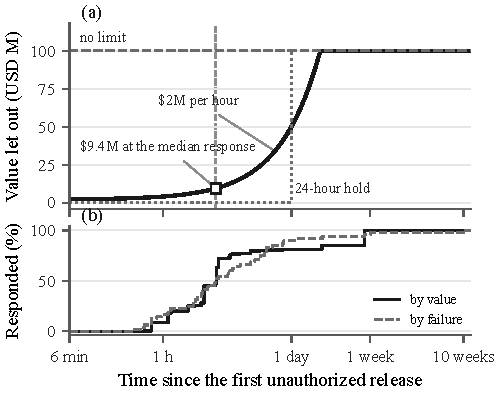
\includegraphics[width=\columnwidth]{figures/fig_example.pdf}
\caption{What a limit lets out, and when responses came. (a) A bridge that holds \$\exHeldM{} million and whose users never withdraw more than \$\exRateM{} million in an hour: no limit (dashed), a token bucket at the release point that refills \$\exRateM{} million per hour and holds \$\exRateM{} million when full (solid; a straight line, bent by the logarithmic axis), and a 24-hour hold on every withdrawal (dotted). The vertical line is the median response time of our failures. (b) Share of the \nTimedEvents{} failures with a recorded response whose first response came by each time, weighted by value and by failure; the second crosses 50\% at the median of panel (a). Logarithmic time axis.}
\label{fig:example}
\end{figure}

\runin{A limit buys time}A limit cannot tell an unauthorized withdrawal from a legitimate one; if it could, the bridge would refuse the first. All it can do is slow every withdrawal down, and it saves money only if someone pauses the bridge before the limit has let the rest out. In Fig.~\ref{fig:example}, a limit of \$\exRateM{} million per hour lets out \$\exLossM{} million of \$\exHeldM{} million by the median response time, and a 24-hour hold on every withdrawal lets out nothing if the response comes within the day and everything if it comes later. The loss is the height of the limit's curve at the moment of the response; we call this curve the limit's exposure curve. Where the limit sits and who controls it, its shape, its numbers and the response time decide that height.

\runin{Where the limit sits}A failure lets withdrawals enter the bridge at some stage and skip the checks before it, and a limit acts only on withdrawals that pass through it. Taken keys and flawed receiving checks let withdrawals in after the verifiers, so a limit in the verifiers' own software sees only forged deposits on the sending chain, failures of the verifiers' own checks, and the redemption of claims minted without backing. On our failures, such a limit could have contained at most \verifierMaxPct\% of the value, whatever its parameters, because that is the share that passed the verifiers. A limit in the contract that releases the funds also sees taken keys and flawed receiving checks, if the verifiers can change neither it nor the pause (Section~\ref{sec:where}); where keys hold the funds directly, there is no such contract. A limit or a pause that the party behind the failure controls can be switched off, and none of the \nRules{} limits we read in source code makes a loosening of its parameters wait.

\runin{What shape it has}Token buckets and windows are ramps, letting out value in proportion to time; a hold on every withdrawal, or a queue that releases itself, is a cliff, letting out nothing until a timer runs out and everything after (Section~\ref{sec:shape}). Every limit that restores its allowance by itself lets everything out if no response comes. A ramp's loss follows the mean response time, and a cliff's loss follows the tail of the response time. A limit that nets deposits against withdrawals adds the other side's limit to its own. A hold on large withdrawals contains nothing by itself against a party that splits them; what it buys is a tighter limit for the rest.

\runin{What numbers to use}Within any time $d$ after a failure, no limit that leaves legitimate users undelayed can let out less than the most that legitimate users ever withdrew within $d$, since the party can replay that traffic. Network calculus gives this floor and the limit that attains it~\cite{leboudec2001}. The floor binds every defense that sees only the amounts and times of withdrawals, including an alarm on the outflow's size or pace. On the traffic of the \pbNWords{} failed bridges that carried \pbValueSharePct\% of the value (Section~\ref{sec:perbridge}), no limit that delays none of a bridge's transfers in the 150 days before its failure could have guaranteed more than \pbFloorPctR\% at the observed response times. Most of the value lost is the 2022 Ronin failure, answered after six days; in the busiest six days of its prior traffic an exchange had withdrawn \$\pbRoninOutsizedM{} million in two transfers, more than the failure took. A limit fitted a month ahead must delay someone as traffic grows. A bucket refitted monthly for a six-hour response keeps \pbBucketPctR\% while delaying \pbBucketDelayedPct\% to \pbBucketDelayedTwoPct\% of legitimate value; about half of that delay is unavoidable (Proposition~\ref{prop:budget}).

\runin{With a check}A check that a deposit backs each release escapes the floor, and the limit behind it is the backstop when the check fails. Matching each release to a deposit by value, the check flags every failure whose withdrawals enter at the verifiers or later, and a forged deposit too, since a forged deposit event moves no value. Used as a gate that holds every withdrawal for \pbGateMin{} minutes while it runs, it stops every failure it flags if a contract holds the funds (Section~\ref{sec:response}). If the check fails, the gate alone keeps nothing and the bucket behind it still keeps \pbBucketPctR\%. Sending only the largest transfer in a thousand to the check spares \pbReviewSparePct\% of transfers the wait and keeps \pbReviewPctR\%, but \pbReviewCheckFailsPct\% if the check fails, since the party's large withdrawals then pass. Such a check paused a testbed bridge within a minute of each injected failure, forged deposits included (Section~\ref{sec:prototype}), and found a deposit behind each of the \shRel{} releases of two live bridges between Ethereum and BSC in 42 days (Section~\ref{sec:response}).

\runin{What the stake must cover}With a limit downstream of the verifiers, and a pause and a confiscation decision they do not control, their stake needs to exceed only what the limit lets out before the response, not the value the bridge holds (Section~\ref{sec:stake}).

\runin{Contributions}\begin{itemize}
\item A dataset of \nEvents{} failures coded by entry stage, control and response and timed where the sources allow, recoded blind from a codebook, and a source-code reading of \nRules{} limits (Section~\ref{sec:bridges}, Appendix~\ref{app:events}).
\item A compact calculus built on network calculus: placement, the exposure curves of deployed limits, a floor set by legitimate traffic that binds every defense seeing only amounts and times, the least delay at a given exposure, and what a check from outside the releases adds (Sections~\ref{sec:model}--\ref{sec:numbers}).
\item Counterfactuals on the failed bridges' own traffic, in sample and a month ahead, with and without the check and with its failure, at their cost to users, on CCIP and on Wormhole, and a consistency check against the \nValidation{} failures that met a deployed limit (Sections~\ref{sec:validation}--\ref{sec:response}).
\item Rules for operators, two prototype limiters, an end-to-end testbed of the check and the pause, and a shadow run of the check on two live bridges (Sections~\ref{sec:response}, \ref{sec:advice} and~\ref{sec:prototype}).
\end{itemize}

\section{Bridges, limits and failures}\label{sec:bridges}

\subsection{How a bridge releases funds}\label{sec:pipeline}

A transfer passes four stages (Fig.~\ref{fig:pipeline}). A user locks or burns an asset on the sending chain, and a contract there emits an event. The bridge's verifiers attest to the event; depending on the bridge they are a validator set, a group of signers, an oracle network or a light client. A contract on the receiving chain checks the attestation and the message. Last, that contract releases the funds: it withdraws an asset from an escrow or a liquidity pool, or it mints a wrapped asset. We call this last stage the release point. A lock-and-mint bridge releases by minting in one direction and from escrow in the other; a liquidity bridge releases from a pool in both. A bridge has many routes, one for each sending chain, release contract and asset.

\begin{figure}[t]
\centering
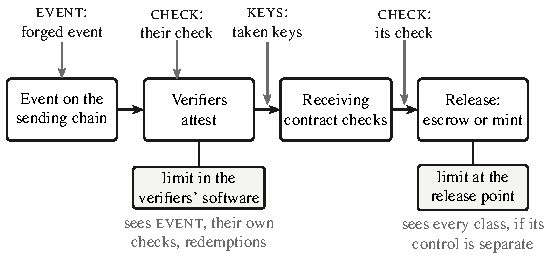
\includegraphics[width=\columnwidth]{figures/fig_pipeline.pdf}
\caption{The four stages of a transfer, and where each class of failure lets unauthorized withdrawals in; a \ccheck{} failure enters after the check that failed, the verifiers' own (left) or the receiving contract's (right). A limit sees a failure only if the failure's withdrawals pass it and the failing party cannot change it: a limit in the verifiers' software sees \cev{} failures, failures of their own checks and the redemption of unbacked mints, and a limit at the release point sees every class if its control is separate from the verifiers.}
\label{fig:pipeline}
\end{figure}

\subsection{Deployed limits}\label{sec:rules}

We read the source code of \nRules{} limits that bridges, messaging protocols and token standards deploy or propose, each at a fixed commit (Table~\ref{tab:rules}); we call each of them a rule. Five properties decide what a rule contains: the stage where it runs, the shape of what it lets out over time, whether it nets inflows against outflows, whether queued withdrawals leave by themselves when a timer runs out, and who controls its parameters and its pause. Of the rules, \nRulesVerifierSideWords{} run in the verifiers' software, \nRulesSendOnlyWords{} acts only on the sending chain, \nRulesReleaseOutsideWords{} act where funds are released (or at the token's mint) under a party other than the verifiers, \nRulesReleasePartlyWords{} more, Axelar's two and Ronin's, have parameters that the verifiers partly govern, and Circle's CCTP is controlled by its verifier. Every on-chain pause takes effect at once. No rule's code delays a loosening of its parameters: a change takes effect at once, or with a node release (Governor) or an upgrade (StarkGate), and the only timelocks sit in the governance above the CCIP and Axelar contracts, each with a path that skips them. \nRulesNoPauseWords{} rules have no pause on releases.

\begin{table*}[t]
\centering
\caption{Limits, read in source code at fixed commits. Stage: verifiers, in the verifiers' software; send, on the sending chain; release, in the contract that releases on the receiving chain; token, in the token contract; send + release, a limit on each side. Shapes as in Table~\ref{tab:shapes}: a ramp lets value out in proportion to time, a cliff all at once when a timer runs out, a geometric limit a fixed share of the balance per period, a bounded limit a fixed total. Accounting: gross counts releases only; net subtracts counted inflows (Section~\ref{sec:shape}). Automatic release: queued withdrawals leave when a timer expires; uncounted means outside the limit. Parameters: who can change the limit; no limit's code delays a loosening. Pause: who can stop releases. Issuer: the token's issuer; operator, owner and governors: a party other than the verifiers. Flow cancelling: inbound transfers offset the cap. Curse: CCIP's stop on releases. RWA: real-world asset.}
\label{tab:rules}
\scriptsize
\setlength{\tabcolsep}{3pt}
\renewcommand{\arraystretch}{1.05}
\begin{tabular}{@{}>{\raggedright\arraybackslash}p{2.95cm} >{\raggedright\arraybackslash}p{1.2cm} >{\raggedright\arraybackslash}p{3.55cm} >{\raggedright\arraybackslash}p{2.95cm} >{\raggedright\arraybackslash}p{1.95cm} >{\raggedright\arraybackslash}p{1.9cm} >{\raggedright\arraybackslash}p{2.0cm}@{}}
\toprule
Limit & Stage & Shape & Accounting & Automatic release & Parameters & Pause \\
\midrule
Wormhole Governor & verifiers & cliff at 24 h (sliding 24 h cap before) & gross (net with flow cancelling) & yes, uncounted & verifiers & any 7 of the 19 verifiers (withhold) \\
Wormhole Global Accountant & verifiers & bounded (releases up to recorded locks) & conservation ledger & no & verifiers & none \\
Wormhole NTT & send + release & ramp; cliff for queued items after 24 h & net (deposits of the same token) & yes, uncounted & issuer & issuer \\
Chainlink CCIP token pools & send + release & ramp (token bucket) & gross & no & issuer & CCIP owner (curse) \\
LayerZero OApp RateLimiter & send & ramp & optional net & no & app owner & app owner \\
LayerZero stablecoin and RWA OFT & send + release & ramp & optional net (deposits of the same token) & no & issuer & sends only \\
Axelar ITS & send + release & ramp (6 h calendar windows) & net within window (deposits of the same token) & no & issuer or operator & operator \\
Axelar legacy gateway & release & ramp (6 h calendar windows) & gross & no & Axelar governance & pauser or governance \\
Hyperlane rate-limited hook and ISM & send or release & ramp & gross & no & route owner & route owner, if added \\
Hyperlane net-flow and delayed-flow & send + release & geometric; cliff at maxDelay for delayed flow & net (deposits of the same token) & delayed flow: yes & route owner & route owner, if added \\
Circle CCTP & send; token & per-message cap at source; bounded at the token & n/a & n/a & verifier (Circle) & verifier (Circle) \\
Linea & send + release & ramp (window from first use; ETH only) & gross & no & operator & operator; council \\
StarkGate & send + release & geometric (5\% of balance per day) & gross within the day & no & operator & none on releases \\
Ronin & release & ramp (UTC day); bounded above the lock threshold & gross & no & bridge admin & admin; pauser \\
Celer cBridge & release & ramp plus delay for large items & gross & yes, counted when queued & governors & pausers \\
Gnosis OmniBridge and xDai & send + release & ramp (UTC day) & gross & no & owner & none (limit to zero) \\
BNB Chain BEP-171 & release & cliff at 12 h & n/a & yes & issuer; governance & validators \\
xERC20 & token & ramp & gross & no & issuer & none (limit to zero) \\
Taiko QuotaManager & release & ramp & gross & no & rollup owner & owner; pauser \\
THORChain outbound delay & verifiers & ramp then cliff & n/a & yes & verifiers & one node \\
THORChain solvency halt & verifiers & bounded (wallet against ledger) & wallet against ledger & auto-resume when solvent & verifiers & automatic \\
ERC-7265 (draft) & release & geometric; cliff in hold mode & net (reported inflow) & hold mode: yes & protocol admin & protocol admin \\
\bottomrule
\end{tabular}
\end{table*}


\runin{The census of CCIP lanes}Of the \ccipEntries{} token lanes configured on Chainlink CCIP~\cite{chainlink_lanes}, \ccipEnabled{} have an outbound token bucket, \ccipInEnabled{} of these also an inbound bucket in the releasing token pool, and the median outbound bucket holds \$\ccipMedCapK{} thousand and refills in \ccipMedRefillH{} hours.

\subsection{Failures}\label{sec:events}

We built a dataset of failures from DefiLlama's list of incidents~\cite{defillama_hacks}, the operators' post-mortems and the chains themselves (Appendix~\ref{app:events}, with the 20 largest in Table~\ref{tab:failures}). Of the \nRecords{} records of at least \$1 million since 2021 that DefiLlama flags as bridge incidents or classes as cross-chain, or that the 2024 systematization lists~\cite{augusto2024sok}, \nEvents{} are unauthorized withdrawals from a bridge's escrow, minting or liquidity, together \$\valueEventsM{} million. We coded each failure by the stage where its withdrawals entered (Fig.~\ref{fig:pipeline}): a forged deposit event on the sending chain (\cev{}, \nClassS{} failures, \classSPct\% of the value), control of the keys that authorize releases (\ckeys{}, \nClassV{}, \classVPct\%), a flaw in a check, in the receiving contract or the verifiers' own software, that accepted a message matching no deposit (\ccheck{}, \nClassD{}, \classDPct\%), and the rest, such as accounting flaws within one chain (\cother{}, \nClassO{}, \classOPct\%). By the side that released, \sideEscrowPct\% of the value left an escrow or a pool, \sideMintPct\% was minted, and \sideBothPct\% was minted on one chain and redeemed from an escrow on another. \nRecovered{} failures saw value returned or frozen later, \recoveredPct\% of the total; we count released value gross and report the net share where it matters. A blind coder, a separate language-model session given a codebook, our descriptions of each failure with the codes removed, and the public sources, agreed on the class of \blindAgree{} of the \nEvents{} failures (Cohen's $\kappa = \blindKappa$); the disagreements carry \blindDisValuePct\% of the value.

We read the times of the first and the last unauthorized release from the chains, and the times of the first public alert by a third party, the operator's first acknowledgment and the pause from the operators' posts or the chains. The first response is the earlier of the acknowledgment and the pause; \nUntimedEvents{} failures, with \$\valueUntimedM{} million in all, have none recorded.

\begin{table}[t]
\centering
\caption{Timing of the failures, measured from the first unauthorized release: median and quartiles over the $n$ failures where each time is known. Last release, 90\% out: a quartile of 0\,s means that at least a quarter of these failures released everything within one block. Alert: the first public alert by a third party. Acknowledgment: the operator's first public statement. First response: the earlier of the acknowledgment and the pause, or for one failure a third party's report that the pause had happened.}
\label{tab:timing}
\footnotesize
\setlength{\tabcolsep}{4pt}
\begin{tabular}{@{}l r r r@{}}
\toprule
Quantity & $n$ & Median & Quartiles \\
\midrule
Last release & 48 & 7\,min 52\,s & 0\,s to 1\,h 8\,min \\
90\% of the value out & 34 & 10\,s & 0\,s to 11\,min 31\,s \\
Alert by a third party & 26 & 1\,h 25\,min & 53\,min 24\,s to 4\,h 2\,min \\
Acknowledgment & 47 & 5\,h 0\,min & 2\,h 35\,min to 12\,h 22\,min \\
Pause & 19 & 3\,h 39\,min & 1\,h 0\,min to 8\,h 9\,min \\
First response & 48 & 3\,h 42\,min & 2\,h 3\,min to 11\,h 23\,min \\
\bottomrule
\end{tabular}
\end{table}


Table~\ref{tab:timing} gives the timing. The releases end within minutes: half of the outflows lasted less than \medOutflowWords{} minutes, and \shareTenMinPct\% of the value left within ten minutes of each failure's first release. The responses came hours later, and \nPausedAfterLast{} of the \nPaused{} pauses came after the last release.

\section{Model}\label{sec:model}

\runin{Limits}A limit $\Lambda$ sits at one stage of one or more routes and acts only on the withdrawals that pass it. At each moment it decides whether to pass each withdrawal on, keep it queued or reject it, using only what happened before. It cannot tell an unauthorized withdrawal from a legitimate one.

\runin{Failures}A deposit \emph{backs} one withdrawal of the value it locked or burned, to the recipient it names; legitimate withdrawals are backed. A failure at time $\tau$ lets an unauthorized party submit unbacked withdrawals that enter at one stage and skip the stages before it, on a set of routes we call its scope, in any amounts and at any times after $\tau$. An \cev{} failure enters before the verifiers, a \ckeys{} failure after them, and a \ccheck{} failure after the check that failed, the verifiers' own or the receiving contract's. The party can take at most $W$: the value held on the routes in scope, or what the claims it can mint are worth on the receiving chain.

\runin{Control and response}A limit or a pause that the party controls through keys or governance rights counts as absent, unless changing it takes longer than the response (Proposition~\ref{prop:timelock}). At time $\tau + D$ a party independent of the failure pauses the release and cancels every queued withdrawal. We call $D$ the response time; if no independent party holds a pause, $D = \infty$. The loss is the party's take in $[\tau, \tau + D)$: what the bridge releases to it less what it deposits.

\runin{Legitimate traffic}Let $\Tset$ be the set of possible legitimate withdrawal histories of the bridge, described by their amounts and times. It is closed under shifts in time and under lowering amounts, to zero included. Its envelope $E(u)$ is the largest legitimate value withdrawn within any window $[s, s + u)$, assumed finite. A limit has delay $h$ if, from its quiet state after a long period without withdrawals, it releases every withdrawal of every history in $\Tset$ within $h$ of its arrival.

\runin{Two measures}The \emph{exposure curve} $\beta_\Lambda(d)$ is the supremum of the party's take within a time $d$ after a failure that $\Lambda$ sees, capped at $W$. It is taken over all strategies of the unauthorized party, from the limit's most permissive state, with no legitimate withdrawal competing for its allowance; the party chooses when to start, so it can wait for that state. For every rule of Table~\ref{tab:rules} the most permissive state is the quiet state: a full bucket, an empty window. The \emph{delay cost} of $\Lambda$ is which legitimate withdrawals wait, and for how long.

\runin{One formula}For a failure answered after a time $D$, the loss satisfies
\begin{equation}\label{eq:loss}
L(D) \le \min\{W, \beta(D)\},
\end{equation}
where $\beta$ is the exposure curve of the limits that the failure's withdrawals pass and that its party cannot switch off; for token buckets, sliding windows and holds the bound is tight (Theorem~\ref{thm:placement}). For a failure that released a value $a$, a limit contains the share $1 - L/a$.

\runin{What the party can do}Besides choosing when to start, the party can split its withdrawals, spread them over the routes in scope, and send deposits through the bridge (Sections~\ref{sec:where} and~\ref{sec:shape}). Until Section~\ref{sec:response}, the way it withdraws does not change the response time, and throughout, it cannot move the prices a limit uses (Proposition~\ref{prop:weights} prices a wrong one).

\section{Where a limit must sit}\label{sec:where}

A limit protects against a failure only if the failure's withdrawals pass through it and the failing party cannot switch it off. In a row of limits every withdrawal passes each of them. Network calculus describes such a row: with the min-plus convolution $(f \otimes g)(d) = \inf_{0 \le s \le d} [f(s) + g(d-s)]$, limits with curves $f$ and $g$ in series let out at most $(f \otimes g)(d)$ within $d$, and a hold for a time $H$ has the curve $\delta_H$, which is $0$ up to $H$ and $+\infty$ after~\cite{leboudec2001}. Call a limit \emph{active} for a failure if it lies on a route in the failure's scope at or after its entry stage, the party does not control it, and for a curve $\beta_j$ with $\beta_j(0) = 0$ it releases by any time $t$ at most what it received by any time $s \le t$ plus $\beta_j(t - s)$.

\begin{theorem}[Placement; concatenation of shapers~\cite{leboudec2001}]\label{thm:placement}
Consider a failure with scope $\mathcal{R}$.
(i) If a route in $\mathcal{R}$ passes no active limit and can release all of $W$, then $L(d) = W$ for every $d > 0$.
(ii) If every route in $\mathcal{R}$ passes at least one active limit of a set $\mathcal{C}$, then $L(d) \le \min\{W, \sum_{j \in \mathcal{C}} \beta_j(d)\}$.
(iii) On a single route with active limits $\beta_1, \dots, \beta_k$ in series,
\begin{equation}\label{eq:placement}
L(d) \le \min\{W, (\beta_1 \otimes \dots \otimes \beta_k)(d)\} \le \min\{W, \min_j \beta_j(d)\}.
\end{equation}
The first bound is tight when the limits are token buckets, sliding windows or holds, and the second is an equality when the curves are concave.
\end{theorem}

The proofs are in Appendix~\ref{app:proofs}, where we also check that every rule of Table~\ref{tab:rules} meets the hypothesis. The second bound in~\eqref{eq:placement} can be strict: a cap of one unit per period followed by a cap of two units per three periods lets out at most $1 + 2 = 3$ units within four periods, while each cap alone would let out four.

\begin{corollary}[Per-channel and pooled limits]\label{cor:pooling}
Let each channel $k$ (a chain's release contract, or an asset) pass its own active limit $\beta_k$ and a pooled active limit $\beta_\Sigma$ common to all. A failure whose scope covers a set $K$ of channels loses at most $\min\{W, \beta_\Sigma(d), \sum_{k \in K} \beta_k(d)\}$ within $d$.
\end{corollary}

A pooled limit stops failures that reach many channels at once, and per-channel limits stop failures confined to one. A pooled limit must sit where every channel's releases pass. Where they leave one contract, such as a token pool that serves many lanes or an escrow that holds many assets, that is the release point. Chains that release from separate contracts can share a pooled limit only through state that the verifiers carry, a stage that misses most failures.

\begin{observation}[Mint side]\label{obs:mint}
A limit only on the escrow of the sending chain does not see an unauthorized mint on the receiving chain. The party sells the minted claims there, and the loss is $W$, their value on the receiving chain; only claims redeemed through the escrow pass the limit.
\end{observation}

A limit can sit downstream of every failure and still be absent if the failing party can change it, as most deployed rules let their owner do at once (Section~\ref{sec:rules}).

\begin{proposition}[Timelocked control]\label{prop:timelock}
Let the party control a limit's parameters, but let a change that loosens them take effect only a time $T$ after it is announced, while the response cancels pending changes and none is pending at $\tau$. Against this party, the limit's exposure curve is $\beta(d)$ for $d \le T$ and $W$ for $d > T$: a cliff at $T$ on top of the limit's own curve. If $D \le T$, the loss is that of a limit the party does not control.
\end{proposition}

\runin{Deployed placements}The Wormhole Governor is a signing policy in the software of the guardians, Wormhole's verifiers~\cite{wormhole_governor}: it sees a forged deposit, but a flawed receiving check bypasses the guardians, and a quorum of guardians whose keys are taken signs without it. A CCIP token pool's inbound bucket sees all three classes, under parameters the token's administrator sets; CCIP's curse, which stops releases, is set by hand by a multisig of Chainlink node operators and Chainlink Labs, an independent pause as far as those signers are not the committee that attests to messages, which we did not check.
\runin{Replay}We replayed each shape of rule at two placements on the \nTimedEvents{} failures with a recorded response, which released \$\valueTimedM{} million (Fig.~\ref{fig:replay}). For a failure that released $a$ and was answered after $D$, the loss under a rule is $\min\{a, k\beta(D)\}$ if the rule sees the failure and $a$ otherwise, where $k$ is the number of chains the failure drained, each with its own copy of the rule (Corollary~\ref{cor:pooling}); Section~\ref{sec:perbridge} fits the rules to each bridge's own traffic. A rule in the verifiers' software sees the \cev{} failures, which carried \$\valueClassSTimedM{} million, the \nVerifierChecksWords{} \ccheck{} failures whose flawed check ran in the verifiers' own software, and the redemption leg of the \nRedeemedLegs{} unbacked mints redeemed through the same bridge, most of the 2022 Wormhole mint among them. A rule at the release point sees the other classes too, except \dFlawReachN{} \ccheck{} failures whose flaw would also have bypassed a limit in the releasing contract, such as an upgrade that removed its checks. We assume, as Section~\ref{sec:advice} recommends, that a party other than the verifiers sets its parameters and holds the pause. As the rules were actually governed, \vKeysCtrlN{} of the \vN{} \ckeys{} failures (\vKeysCtrlValuePct\% of the value) used keys that also controlled the releasing contract, and the rule would not have seen them. In \keysHeldN{} failures, \keysHeldPct\% of the value, keys held the custody directly, with no contract that could hold a limit; there a limit can run only in the signers' software, which sees what a verifier-side limit sees.

Whatever its shape and parameters, a rule in the verifiers' software would have contained at most \verifierMaxPct\% of the value. At the release point, a token bucket of \$1 million per hour would have contained \plRampSepPct\% (\plRampGovPct\% as governed, \plRampContractPct\% with custody held by keys limited in the signers' software) and a 24-hour hold \plHoldSepPct\% (\plHoldGovPct\%; \plHoldContractPct\%). The verifier-side ceiling is the share that passed the verifiers, so it rests on the coding: under the readings that the post-mortems leave open, it lies between \ceilLowPct\% and \ceilHighPct\% (Appendix~\ref{app:events}), the blind coder's reading of the legs gives \blindVerifierPct\%, and without the three largest failures, none of which passed the verifiers, it is \verifierCeilNoTopThreePct\%.

\begin{figure}[t]
\centering
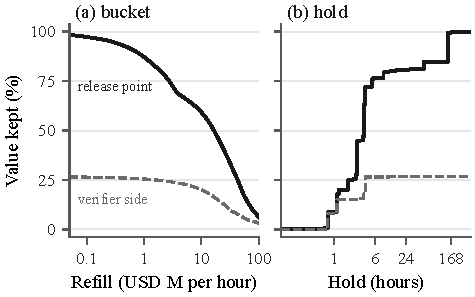
\includegraphics[width=\columnwidth]{figures/fig_replay.pdf}
\caption{Share of the value of the \nTimedEvents{} failures with a recorded response that a rule would have contained, at the release point (solid) and in the verifiers' software (dashed), with the response times as observed. (a) Token bucket with refill $r$ and a capacity of one hour of refill, one for each chain a failure drained. (b) Hold on every withdrawal for $H$, cancelled by the response.}
\label{fig:replay}
\end{figure}

\section{What shape a limit has}\label{sec:shape}

The shape of the exposure curve decides how the loss grows with the response time (Table~\ref{tab:shapes}).

\begin{table}[t]
\centering
\caption{Exposure curves of the deployed families from the most permissive state, capped at $W$. $N(d)$: messages processed within $d$; $n(d) = \lceil d/w \rceil + 1$: calendar windows touched within $d$; $\beta_0$: the rule's curve under an automatic release after $A$; $\beta_B$: the curve on the side that pays deposits back.}
\label{tab:shapes}
\footnotesize
\setlength{\tabcolsep}{3pt}
\begin{tabular}{@{}l l l@{}}
\toprule
Rule & $\beta(d)$ & Shape \\
\midrule
Cap $C$ per message & $C\,N(d)$ & throughput \\
Sliding window, $C$ per $w$ & $C \lceil d/w \rceil$ & ramp \\
Calendar window, $C$ per $w$ & $C\,n(d)$ & ramp \\
Token bucket $(b, r)$ & $b + r d$ & ramp \\
Hold $H$, cancellable & $0$ for $d \le H$, else $W$ & cliff \\
Hold $H$, then bucket & $(b + r(d - H))\,\mathbf{1}[d > H]$ & ramp \\
Automatic release after $A$ & $\beta_0(d)$ for $d \le A$, else $W$ & cliff \\
Share $p$ of balance per window & $W\bigl(1 - (1-p)^{n(d)}\bigr)$ & geometric \\
Bucket netting deposits & $b + rd + \beta_B(d)$ & ramp \\
Net flow, forged inflows, no cap & $W$ & immediate \\
Cumulative cap $\theta$, reviewed & $\theta$ & bounded \\
\bottomrule
\end{tabular}
\end{table}

\begin{proposition}[Deployed families]\label{prop:families}
Each rule of Table~\ref{tab:shapes} has the exposure curve listed there if the party's deposits leave a balance share's base unchanged and no review resets the cumulative cap before the response.
\end{proposition}

A calendar window lets its full cap out just before a boundary and again just after it, so its curve starts at twice the cap. The last column has six shapes; Observation~\ref{obs:regeneration} and Proposition~\ref{prop:netflow} explain why only one of them is bounded.

\begin{observation}[Regeneration]\label{obs:regeneration}
Suppose that after every period of some length without releases a rule restores at least a fixed amount or a fixed share of what remains, with no action by a person or by a party independent of the failure: by a refill, a window that slides or resets, a timer that releases a queue, or a new window of a balance share. If no response comes, then $\sup_d \beta(d) = W$.
\end{observation}

Every ramp, cliff and geometric rule therefore buys time and nothing more. A bound that does not depend on the response time needs an allowance that does not come back by itself, as in a cumulative cap that resets only after a review, which stops legitimate traffic each time it has moved $\theta$.

\begin{proposition}[Net flow across both sides]\label{prop:netflow}
Let a rule on side $A$ of a bridge let out within $d$ at most $\beta_A(d)$ plus the inflows $I(d)$ it counts, with $W$ counting the value on both sides.
(i) If each counted unit of inflow costs the party $c$ in value it does not get back, its take within $d$ is at most $\min\{W, \beta_A(d) + (1-c) I(d)\}$: as tight as $\beta_A$ for $c \ge 1$, and growing with $I$ for $c < 1$.
(ii) If the counted inflows are deposits of the same token that the bridge pays back to the party on side $B$ through active limits with curve $\beta_B$, the take is at most $\min\{W, \beta_A(d) + \beta_B(d)\}$; if counted deposits restore $A$'s allowance at once, $A$ lets something out from its quiet state and both curves are reached from a common start, the party approaches it without capital of its own, up to the time a deposit takes to be paid out.
\end{proposition}

Of the \nRulesNetWords{} rules besides the Governor that net inflows, \nRulesNetSameTokenWords{} count deposits of the same token. Axelar's flow limits and the LayerZero stablecoin option reject the matching release above the other side's limit, so they add it; NTT releases the matching transfer after 24 hours without counting it, and Hyperlane's net-flow rule does not limit the matching mint, so there the round trip is bounded only by the party's time. StarkGate counts deposits in the next day's balance, so it too nets them, a day late. The Governor's flow cancelling counts transfers that the guardians attest, which a \cev{} failure on the partner chain fabricates at no cost ($c = 0$), up to that chain's own cap.

\begin{proposition}[Holds by observable class]\label{prop:split}
Let a rule hold until a review every withdrawal in a class $\mathcal{K}$ defined by observable features, such as a size above $s$, a destination or an anomaly score, and pass the others through a limit $\Lambda$.
(i) Against a party that can keep its withdrawals outside $\mathcal{K}$ at no cost, the rule's exposure curve is at most $\beta_\Lambda$, with equality for a class of large withdrawals and a bucket or window $\Lambda$.
(ii) $\Lambda$ needs to pass only legitimate traffic outside $\mathcal{K}$, so with delay $h$ it can be as tight as $E_{\bar{\mathcal{K}}}((d-h)^+)$, where $E_{\bar{\mathcal{K}}}$ is the envelope of that traffic.
(iii) If held withdrawals are released by a timer after $A$ instead of a review and the party can submit $W$ in $\mathcal{K}$, the curve is at most $\max\{\beta_\Lambda(d), W\,\mathbf{1}[d > A]\}$, a cliff, with equality as in (i).
\end{proposition}

A hold on large withdrawals therefore contains nothing by itself against a party that can split below $s$ at no cost; what it buys is the tighter limit for small ones. Sections~\ref{sec:perbridge} and~\ref{sec:ccip} measure that gain.

\begin{observation}[Mean and tail]\label{obs:meantail}
Let the response time $D > 0$ have distribution $G$. A token bucket that lets out less than $W$ within every response time loses $b + r\,\mathbb{E}_G[D]$ on average, and a hold for $H$ loses $W \Pr_G(D > H)$.
\end{observation}

\runin{Replay}At the release point, a token bucket would have contained \rampPointOneMPct\% of the value with a refill of \$0.1 million per hour and \rampThirtyMPct\% with \$30 million per hour (Fig.~\ref{fig:replay}). A hold would have contained \cliffOneHPct\% with a deadline of one hour, \cliffSixHPct\% with six hours and \cliffDayPct\% with a day; a longer deadline adds little (\cliffThreeDPct\% at three days), because most of the late value is the 2022 Ronin failure, answered after six days. These shares keep each response time as observed. A hold also postpones the outflow through which \outflowDetectedN{} failures were found; if their response came only after the hold released them, the 24-hour hold would contain \rtHoldOutflowPct\%. Weighted by failure, the hold contains \wtHoldEventPct\% and the bucket \wtRampEventPct\%: a hold stops small failures as fully as large ones, a ramp mostly the large. Net of the value later returned or frozen, the bucket contains \wtRampNetPct\% and the hold \wtHoldNetPct\%.

\section{Failures that met a limit}\label{sec:validation}

Of the \nEvents{} failures, \nValidationWords{} met a rule in force that limits, holds or pauses releases. Table~\ref{tab:validation} gives what the model predicts from the rule's placement, control and shape, and what happened. We wrote the predictions knowing the outcomes, so this checks consistency rather than testing the model; two predictions are amounts that the chain can check.

\begin{table}[t]
\centering
\caption{Failures that met a rule in force. Prediction: what the model says the rule could hold, from its placement, control and shape (Sections~\ref{sec:where} and~\ref{sec:shape}); for the first three rules, at the release point under separate control, the bound from the parameters in force and the time the outflow ran. Outcome: what the failure released (Appendix~\ref{app:events}).}
\label{tab:validation}
\scriptsize
\setlength{\tabcolsep}{2.5pt}
\begin{tabular}{@{}>{\raggedright\arraybackslash}p{1.42cm} >{\raggedright\arraybackslash}p{2.0cm} >{\raggedright\arraybackslash}p{2.3cm} >{\raggedright\arraybackslash}p{2.3cm}@{}}
\toprule
Failure & Rule in force & Prediction & Outcome \\
\midrule
Taiko (2026) & ether quota of 1,000 a day, 999 used before & at most 297 ether by the last release (41.7 an hour) & 278 ether (94\%); assets without a quota in full \\
Ronin (2024) & review above 4,000 ether or 2M USDC; daily cap & at most 4,397 ether and 2.48M USDC & 3,996 ether (91\%), 2.00M USDC (80\%) \\
Poly Network Neo (2024) & a fifth of the backing in the releasing contract & at most that contract's balance & ended when it was empty \\
Nomad (2022) & 30-minute window on new message roots & a hold in a skipped stage holds nothing & root accepted at initialization \\
THORChain (2026) & halt of the verifiers' signing & a halt there misses key-signed releases & key-signed releases went on \\
QANplatform (2022) & cap per transaction for each signer & a cap the failing key controls is absent & cap set to the maximum \\
ChainSwap (2021) & quota per signer & a cap per message does not bound the total & 1,136 releases in 35 minutes \\
Maya Protocol (2026) & delay for large outbound transfers & a delay by size holds nothing below it & no outbound was delayed \\
AFX Trade (2026) & 200-second dispute window & a cliff holds nothing after its deadline & elapsed unchallenged \\
Aztec 2.0 (2026) & escape window of 48 minutes in 16 hours & an open window without a cap holds nothing & all releases in an open window \\
NEAR Intents (2026) & outlier monitor that pauses & an alarm alone saves what is left & paused after the last release \\
Shibarium (2025) & halt on inconsistent checkpoints & an alarm alone saves what is left & halted after both releases \\
Nomic on Osmosis (2026) & static cap on a pool's share & a cap whose room returns lets all out & 18 of 40.65 on day one; the rest later \\
\bottomrule
\end{tabular}
\end{table}


The Taiko bridge gave ether a quota of \valTaikoQuota{} a day that refilled at \valTaikoRate{} an hour. Three hours before the first release, a processed message counted \valTaikoUsed{} ether against the quota but moved none, so with the refill the model bounds the ether released by the last release, four hours after the first, at \valTaikoBound{}; the contract's own reading just before the first release, \valTaikoRead{} ether available, matches the refill formula. \valTaikoOut{} ether left in small releases at the pace of the refill, \valTaikoPct\% of the bound and never above it; assets without a quota left in full. In the 2024 Ronin failure, withdrawals above \valRoninEthLock{} ether or \valRoninUsdcLockM{} million USDC were locked for review, and those below counted against a daily cap of \valRoninEthDaily{} ether and \valRoninUsdcDailyM{} million USDC, partly used that day, so a party that avoids the lock takes at most \valRoninEthBound{} ether and \valRoninUsdcBoundM{} million USDC. It took \valRoninEthOut{} ether (\valRoninEthPct\%) and \valRoninUsdcOutM{} million USDC (\valRoninUsdcPct\%), one withdrawal each just below the lock size, as Proposition~\ref{prop:split} predicts. Poly Network's Neo route kept about a fifth of its backing in the contract that released, and the outflow on Ethereum ended when that contract was empty. The other ten predictions follow from placement and control alone: the rule sat in a stage the failure skipped or under the failing key, held nothing below its size, or gave out before the response, as Observation~\ref{obs:regeneration} predicts for the cap on Osmosis.

\section{Setting the numbers}\label{sec:numbers}

A limit's numbers trade the loss at the response time against the delay of legitimate users, and legitimate traffic sets a floor under the trade.

\begin{theorem}[Floor; minimal arrival curve and greedy shaper~\cite{leboudec2001}]\label{thm:floor}
(i) If a limit $\Lambda$ has delay $h$, then $\beta_\Lambda(d) \ge \min\{W, E((d-h)^+)\}$ for every $d$. The limit $\Lambda^*$ that holds each withdrawal for $h$ and then releases greedily, so that no window of length $u$ releases more than $E(u)$, has delay $h$ and $\beta_{\Lambda^*}(d) = \min\{W, E((d-h)^+)\}$.
(ii) The bound in (i) holds for any defense that decides when to release and whether to pause using only the amounts and times of the withdrawals it receives and of its own releases, such as a limit with an alarm on the size or pace of releases, if from its quiet state it releases every history in $\Tset$ within $h$ of each arrival and pauses none. If instead it pauses each history in $\Tset$ within $d$ with probability at most $\alpha$ and otherwise releases it within $h$ of each arrival, its expected loss within $d$ is at least $(1-\alpha)\min\{W, E((d-h)^+)\}$.
(iii) If a party independent of the failure pauses within $\ell$ of the first withdrawal that no deposit backs, the loss with a limit $\Lambda$ is at most $\min\{W, \beta_\Lambda(\min\{d, \ell\})\}$. If every withdrawal is first held for $H \ge \ell$, such a failure loses nothing, and one whose withdrawals the check passes loses at most $\min\{W, \beta_\Lambda((d-H)^+)\}$.
\end{theorem}

The unauthorized party can replay the busiest legitimate window, and a limit that lets every legitimate history through within $h$ must let that replay through as well; so must any defense that sees only amounts and times, since the replay looks legitimate to it, and a detector that pauses at random escapes only by its false-alarm probability. A defense that also uses what the party cannot copy, such as the history of recipients or the call structure of a transaction, as transaction-level detectors do~\cite{wu2025bridgeguard,lin2025bridgeshield}, escapes the floor as far as those features separate the two, at the cost of the legitimate withdrawals it flags. Information from outside the releases, the deposits on the sending chain, escapes it entirely; part~(iii) gives the price, a hold on every withdrawal, and Section~\ref{sec:response} evaluates it. With $h = 0$, no limit that never delays a legitimate user can lose less than $\min\{W, E(D)\}$, the most that legitimate users ever withdrew within a response time. A failure smaller than that passes under every such limit, so limits protect against large failures. Since $\Lambda^*$ attains the floor at every $d$, it has the smallest exposure among limits of delay $h$ at every response time at once.

\begin{proposition}[Delay budget]\label{prop:budget}
Let $d > h$, and let a defense as in Theorem~\ref{thm:floor}(ii) let out at most $x$ within any interval of length $d$. On every legitimate history $\ell$, it delays by more than $h$ a value of at least $F(x) = \sup \sum_k (\ell(I_k) - x)^+$, the supremum over disjoint intervals $I_k$ of length $d-h$.
\end{proposition}

A sliding window of length $w$ with cap $E(w)$ delays no legitimate history but lets out $\min\{W, E(w)\}$ within any $d \in (0, w]$ (Corollary~\ref{cor:windows}): a daily cap set at the busiest legitimate day lets out $\min\{W, E(24\,\mathrm{h})\}$ in a failure answered within an hour.

\begin{proposition}[One token bucket; burstiness curve]\label{prop:hull}
A token bucket with capacity $b$ and refill $r$ has delay zero if and only if $b \ge B(r) = \sup_u [E(u) - ru]$. Among these buckets the smallest budget $b + rD$ for a response time $D > 0$ is $\hat{E}(D) = \min_r [B(r) + rD]$, where $\hat{E}$ is the least concave majorant of $E$, and the bucket whose line supports $\hat{E}$ at $D$ attains it.
\end{proposition}

A bucket's parameters should therefore follow the response time it is meant for. Averaged over uncertain response times, the bucket that supports $\hat{E}$ at the mean has the smallest budget (Proposition~\ref{prop:mean}), but the loss is capped at $W$, and when $W$ binds for long responses the best bucket supports $\hat{E}$ at a shorter time: on Wormhole's combined traffic with $W = \$1$ billion, at \bestOneBDStarH{} hours, against a mean response of \meanRespH{} hours. One bucket gives up little: on CCIP lanes the median of $\hat{E}(D)/E(D)$ is \oneBucketCcipOneMed{} at one hour and \oneBucketCcipSixMed{} at six hours.

\begin{observation}[Several buckets]\label{obs:kbuckets}
Token buckets in series, each supporting $\hat{E}$ at one of $D_1 < \dots < D_K$, delay no legitimate history and let out at most $\min_k (b_k + r_k d)$ within $d$, which equals $\hat{E}(D_k)$ at each $D_k$.
\end{observation}

On Wormhole's combined traffic, four buckets matched to one hour, six hours, a day and a week stay within \kBucketsHullPct\% of $\hat{E}$ and \kBucketsEnvPct\% of the floor $E$ from one hour to 30 days, so an operator can approach $\Lambda^*$ without an estimate of $D$.

\subsection{The failed bridges' own traffic}\label{sec:perbridge}

We rebuilt the legitimate releases of failed bridges over the 150 days before each failure, from the events of their release contracts, and priced them in dollars (Appendix~\ref{app:methods}): \pbSelectionText{} The totals cover \pbNWords{} failures, which carried \pbValueSharePct\% of all the value; \pbApartText{} Every release contract of a bridge gets its own limit, with its assets pooled in dollars, and a failure is charged the sum over the contracts in its scope (Corollary~\ref{cor:pooling}); for every failure here with several contracts, the taken keys or the flaw reached all of them. The floor, $\Lambda^*$ with $h = 0$ fitted in sample, delays none of the 150 days, so it is the most a limit delaying none of that history could have guaranteed against a party pacing itself like the busiest legitimate traffic; it is a best case, not a design. The bucket is fitted out of sample, as a monthly refit would fit it: to the 90 days that end 30 days before the failure, for a six-hour response with a margin of 1.5 (Proposition~\ref{prop:hull}), with its cost measured on the 30 days that follow, \pbTestTransfers{} transfers in all, and again one month earlier.

\begin{table*}[t]
\centering
\caption{Limits fitted to each failed bridge's own traffic before the failure: share of the value released in the failure that each would have kept at the response time $D$. Legit: legitimate value released per day over the 150 days before the failure. Floor: the limit shaped like all 150 days, fitted in sample, which delays none of them; it is the most a limit that delays no legitimate transfer of that history could keep. Bucket: a token bucket fitted out of sample to the 90 days that end 30 days before the failure, for $D = 6$\,h, with a margin of 1.5. Review: transfers above the 99.9th percentile of sizes in those 90 days wait for a review that the party cannot pass, and a bucket for $D = 1$\,h with a margin of 1.5 takes the rest. Alarm: a pause one hour after the first release that no deposit backs, with the review design or alone, where the check flags the failure and someone other than the failing party can stop it. A range: the value released within the first hour is known only between bounds. Each release contract that a failure reaches has its own limit. Net: weighted by the value never returned or frozen. $^\dagger$Left out of the totals (Section~\ref{sec:perbridge}). Table~\ref{tab:pbcost} gives what the designs cost legitimate users and keep when the check fails.}
\label{tab:perbridge}
\footnotesize
\setlength{\tabcolsep}{4pt}
\begin{tabular}{@{}l l l r r r r r r r r@{}}
\toprule
 & & & & & & \multicolumn{5}{c}{Kept at $D$}  \\
\cmidrule(l){7-11}
 & & & & & & In sample & \multicolumn{2}{c}{Out of sample} & \multicolumn{2}{c}{Alarm in 1\,h}  \\
\cmidrule(lr){7-7} \cmidrule(lr){8-9} \cmidrule(l){10-11}
Failure & Year & Class & \$M & $D$ (h) & Legit (\$M/day) & Floor & Bucket & Review & Review & Alone \\
\midrule
Poly Network & 2021 & flaw & 610 & 2.8 & 14.06 & 83\% & 82\% & 92\% & 95\% & 0\% \\
BSC Token Hub & 2022 & flaw & 587 & 3.8 & 2.72 & 96\% & 94\% & 100\% & 100\% & 50\% \\
Ronin 2022 & 2022 & keys & 540 & 145.9 & 24.27 & 0\% & 0\% & 0\% & 90\% & 0\% \\
Wormhole & 2022 & flaw & 322 & 1.1 & 5.98 & 65\% & 95\% & 96\% & 96\% & 0\% \\
Liquid & 2026 & event & 318 & 4.0 & 1.07 & 98\% & 99\% & 99\% & 100\% & 0\% \\
Kelp rsETH & 2026 & flaw & 294 & 0.8 & 3.12 & 95\% & 84\% & 93\% & 93\% & 0\% \\
Nomad & 2022 & flaw & 187 & 1.9 & 1.15 & 89\% & 93\% & 98\% & 99\% & 85\% \\
Multichain 2023 & 2023 & keys & 129 & 5.3 & 1.53 & 86\% & 75\% & 81\% & 89\% & 15\% \\
Harmony Horizon & 2022 & keys & 100 & 8.8 & 5.08 & 12\% & 0\% & 35\% & 72\% & 1--2\% \\
HECO bridge & 2023 & keys & 86 & 2.6 & 0.38 & 90\% & 84\% & 90\% & 90\% & 0\% \\
Orbit Bridge & 2023 & keys & 82 & 1.2 & 0.31 & 98\% & 95\% & 97\% & 98\% & 0\% \\
Qubit QBridge$^\dagger$ & 2022 & event & 80 & 3.6 & 0.01 & 99\% & 99\% & 100\% & 100\% & 0\% \\
AFX bridge$^\dagger$ & 2026 & keys & 24 & 5.6 & 0.02 & 99\% & 99\% & 99\% & 99\% & 0\% \\
Wanchain Cardano & 2026 & flaw & 14 & 15.1 & $<$0.01 & 100\% & 100\% & 100\% & 100\% & 0\% \\
Ronin 2024$^\dagger$ & 2024 & flaw & 12 & 0.6 & 1.37 & 0\% & 0\% & 79\% & 79\% & 0\% \\
Poly Network 2023 & 2023 & keys & 10 & 6.8 & 0.21 & 40\% & 15\% & 36\% & 55\% & 0--10\% \\
Syscoin bridge & 2026 & flaw & 9 & 11.1 & $<$0.01 & 100\% & 100\% & 100\% & 100\% & 0\% \\
Anyswap V3 router$^\dagger$ & 2021 & keys & 8 & 19.5 & 0.53 & 0\% & 87\% & 86\% & 97\% & 0\% \\
Verus bridge July & 2026 & flaw & 8 & 0.6 & 0.02 & 96\% & 97\% & 98\% & 98\% & 0\% \\
Gravity Bridge & 2026 & event & 5 & 11.0 & $<$0.01 & 97\% & 100\% & 100\% & 100\% & 0\% \\
\midrule
By value (sixteen failures) & & & & & & 71\% & 72\% & 78\% & 94\% & 14\% \\
\quad 90\% bootstrap interval & & & & & & 49--90 & 49--90 & 53--96 & 92--97 &  \\
By failure & & & & & & 78\% & 76\% & 82\% & 92\% & 9\% \\
Net & & & & & & 57\% & 57\% & 63\% & 92\% &  \\
\bottomrule
\end{tabular}
\end{table*}


\runin{In sample}The floor keeps \pbFloorPct\% of the value (\pbFloorEventPct\% averaged over failures; \pbFloorLoPct--\pbFloorHiPct\% over bootstrap samples of the failures and \pbFloorLooLoPct--\pbFloorLooHiPct\% leaving one out). Most of the loss is the 2022 Ronin failure, answered after six days: the busiest six days of Ronin's prior traffic released \$\pbRoninEnvM{} million, more than the \$\pbRoninTakenM{} million taken, \$\pbRoninOutsizedM{} million of it in two withdrawals three days apart to wallets that public labels assign to one exchange. Without those two, Ronin's floor keeps \pbRoninFloorTrimPct\% and the total \pbVarFloorPct\%. On the other \pbOthersN{} failures the floor keeps \pbOthersFloorPct\%.

\runin{Out of sample}A limit fitted to the past must delay users when traffic grows. The bucket keeps \pbBucketPct\% (\pbBucketLoPct--\pbBucketHiPct\%), but it delayed \pbBucketDelayedPct\% of legitimate value in the month before the failures and \pbBucketDelayedTwoPct\% in the month before that, \pbBucketCountPct\% and \pbBucketCountTwoPct\% of the transfers. About half of that delay is unavoidable: no defense that lets out as little within six hours could have delayed less than \dbLowerPct\% and \dbLowerTwoPct\% (Proposition~\ref{prop:budget}). Matched to one hour, a day or 50 hours instead of six, it keeps \pbBucketOnePct\%, \pbBucketDayPct\% and \pbBucketFiftyPct\% and delays \pbBucketOneDelayedPct\%, \pbBucketDayDelayedPct\% and \pbBucketFiftyDelayedPct\%: the cap binds for slow responses, so a short design time loses nothing there.

A review takes the transfers that a bucket fitted to the past cannot absorb. Sending transfers above the 99.9th percentile of the fit window's sizes to a review, and matching a bucket for the rest to one hour (Proposition~\ref{prop:split}), keeps \pbReviewPct\% (\pbReviewLoPct--\pbReviewHiPct\%), and that bucket delays only \pbReviewDelayedPct\% and \pbReviewDelayedTwoPct\% of legitimate value. The reviewed transfers are few and large: a median of \pbReviewPerMonthMed{} per bridge and month and at most \pbReviewPerMonthMax{}, carrying \pbReviewSharePct\% and \pbReviewShareTwoPct\% of legitimate value. With reviews that take an hour, legitimate value waits \pbReviewWaitOneH{} to \pbReviewWaitOneHTwo{} hours per dollar, and with a day, \pbReviewWaitDayH{} to \pbReviewWaitDayHTwo{} hours; by hand they are slow, and the \roninReviewN{} withdrawals that Ronin's gateway has held for review since 2022 waited a median of \roninReviewMedH{} hours. A review protects only if the party cannot pass it, so it must check what the party cannot fake; Section~\ref{sec:response} takes it to be the check that a deposit backs the release and asks what remains when that check fails.

\runin{Robustness}On Poly Network, \pbPolyUnpricedPct\% of the releases in 2021 and \pbPolyTwoUnpricedPct\% in 2023 could not be priced, so its limits overstate what they keep. As governed, with the \ckeys{} failures whose keys controlled the release contract left unseen, the bucket keeps \pbBucketGovPct\% and the review design \pbReviewGovPct\%; with custody held by keys limited in the signers' software, \pbBucketKeysHeldPct\% and \pbReviewKeysHeldPct\%; on the \pbPauseFirstN{} failures whose first response was a pause, \pbPauseFirstBucketPct\% and \pbPauseFirstReviewPct\%; with response times five times longer, \pbBucketFivePct\% and \pbReviewFivePct\%; weighted by the value never returned or frozen, \pbBucketNetPct\% and \pbReviewNetPct\%. Fitted to 60 or 120 days, the review design keeps \pbWinReviewPct\%.

\subsection{Chainlink CCIP}\label{sec:ccip}

\runin{Today's buckets}Of the \ccipSelLanes{} CCIP lanes that carried the most value from January to October 2026 (\ccipSelSharePct\% of it; Appendix~\ref{app:methods}), \ccipMisLanes{} have an inbound bucket. Its release within $D$, divided by $\hat{E}(D)$ from the lane's own history, ranges from \ccipInRatioMinOne{} to \ccipInRatioMaxOne{} at $D = 1$\,h and from \ccipInRatioMinSix{} to \ccipInRatioMaxSix{} at $D = 6$\,h; it is above one, looser than the traffic needs, on \ccipInLooseOne{} and \ccipInLooseSix{} lanes. Every observed transfer passed the limits in force: a transfer above a bucket is rejected and leaves no record, one lane's traffic traces its outbound bucket, and on \ccipLanesDisabledHalf{} of the \ccipInLanes{} lanes of Table~\ref{tab:ccip} (one lane has too short a history for it) more than half the value moved while the bucket was disabled. Replaying today's buckets therefore measures what these numbers would cost, not what users paid.

\runin{A schedule}Fitted to the first half of a lane's history, a bucket delays nothing in the second half on \ccipOosZero{} of the \ccipOosLanes{} lanes, and up to \ccipOosMaxPct\% of the value where traffic grew. We therefore evaluated a schedule that every 30 days refits the bucket to the previous 90 days for a response time $D$ and scales it by a margin $\mu$ (Table~\ref{tab:ccip}; transfers queue in order of arrival).

\begin{table}[t]
\centering
\caption{Inbound buckets at the release point of 16 CCIP token lanes, replayed on execution times in 30-day segments against today's buckets. Each 30 days, a bucket is refitted to the previous 90 days for a response time $D$ (in hours) and scaled by a margin $\mu$. Review: transfers above the 99th percentile of sizes in the fit window, about 2.4 per lane and month, wait for a review, and the bucket is fitted to the rest. Delayed: share of value that the bucket delayed. Delay: hours of waiting in the bucket per dollar of tested value. Reviewed: share of value sent to review. Even: the review latency, in hours, at which the delay per dollar, counting a reviewed transfer as waiting that latency, equals today's. 1\,h, 6\,h: release within that time, median over lanes, relative to today's bucket.}
\label{tab:ccip}
\footnotesize
\setlength{\tabcolsep}{2.6pt}
\begin{tabular}{@{}l l l r r r r r r@{}}
\toprule
$D$ & $\mu$ & Review & Delayed & Delay & Reviewed & Even & 1\,h & 6\,h \\
\midrule
\multicolumn{3}{@{}l}{Today's buckets} & 19.3\% & 0.53 & -- & -- & 1 & 1 \\
6 & 1.5 & no & 8.3\% & 10.76 & -- & -- & 1.57 & 0.60 \\
1 & 1.5 & no & 9.7\% & 9.90 & -- & -- & 1.18 & 0.99 \\
1 & 1 & yes & 4.9\% & 0.12 & 24\% & 1.7 & 0.42 & 0.35 \\
1 & 1.5 & yes & 0.8\% & 0.01 & 24\% & 2.2 & 0.62 & 0.52 \\
1 & 2 & yes & 0.0\% & 0.00 & 24\% & 2.2 & 0.83 & 0.70 \\
6 & 1.5 & yes & 3.6\% & 0.34 & 24\% & 0.8 & 1.09 & 0.44 \\
6 & 2 & yes & 0.7\% & 0.04 & 24\% & 2.1 & 1.46 & 0.58 \\
\bottomrule
\end{tabular}
\end{table}


Matched to six hours with $\mu = 1.5$, the schedule delays \ccipNoRevDelayedPct\% of legitimate value against \ccipInTodayDelayedPct\% for today's buckets, but a few transfers larger than anything in the fit window wait a median of \ccipNoRevWaitPFifty{} hours; operators pass such transfers today by raising the limit by hand. Sending transfers above the 99th percentile of the fit window's sizes to a review and matching the bucket for the rest to one hour removes them: the bucket then delays \ccipRevDelayedPct\% of the value, the release within one and six hours falls to \ccipRevCapOne{} and \ccipRevCapSix{} of today's on the median lane, and \ccipRevPerMonth{} transfers per lane and month, \ccipRevValuePct\% of the value, wait for a review. This variant delays legitimate value less than today's buckets, \ccipInTodayMeanDelayH{} hours per dollar, if reviews take less than \ccipRevBreakevenH{} hours. \ccipRevLowerBoth{} of the \ccipRevVariants{} review variants we tried release less than today's buckets at both response times, with break-even latencies of \ccipRevBreakevenMinH{} to \ccipRevBreakevenMaxH{} hours.

\subsection{Pooling across chains and assets}\label{sec:pooling}

Most failures are confined: \nSingleChain{} of the \nEvents{} released value on one chain, and against them pooling helps only in series with per-chain caps (Corollary~\ref{cor:pooling}). Against a failure that reaches every chain it helps a lot: over twelve months, across the \wormChainsWords{} main chains of Wormhole's token bridge, caps sized to each chain let out \poolLow{} to \poolHigh{} times what one pooled cap would, for windows from one hour to one day. Large transfers dominate short windows: without the \wormBigTwelveN{} transfers above the Governor's size threshold, \wormBigTwelveValuePct\% of the value, the one-hour envelope of the combined traffic falls by a factor of \wormEnvRatio{}, to \$\wormEnvOneHSmallM{} million. The Governor's daily caps seldom delay small transfers: over 24 months the trailing 24-hour outflow exceeded the cap in \govSuiHours{} hours on Sui and in at most \govOtherMaxHours{} on any other chain. A pooled limit meters assets at weights in a common unit, and a weight that undervalues an asset by a factor $x$ loosens the limit for it by that factor, which a cap on each asset bounds (Proposition~\ref{prop:weights}); the Governor, which takes the larger of a configured and the market price, undervalues only when its feed fails and the price has risen.

\section{The response and the check}\label{sec:response}

The shares so far take each failure's first public response as given, and for \nRespAck{} of the \nTimedEvents{} failures it is an acknowledgment. Where both an acknowledgment and a pause are recorded, the pause came first in \respPauseFirstN{} of \respBothN{}, by a median of \respAckAfterPauseH{} hours, so an acknowledgment more likely overstates the time to the pause than understates it; \respPauseOnchainN{} pauses are timed from the chain. We found no difference in response times between weekends and weekdays ($p = \respWeekendP$) or across the hours of the day ($p = \respHourP$), and they have not become faster: medians of \respEarlyMedH{} hours for the \respEarlyN{} failures of 2021 to 2023 and \respLateMedH{} hours for the \respLateN{} of 2024 to 2026.

A limit could change response times in both directions. A party paced by a limit withdraws at the pace of busy legitimate traffic, which hides the outflow through which \outflowDetectedN{} of the \nEvents{} failures, with \outflowDetectedValuePct\% of the value, were found. If none of them had been answered, a bucket of \$1 million per hour would still have contained \rtRampOutflowPct\% of the value, and the bucket fitted in Section~\ref{sec:perbridge}, \pbBucketOutflowPct\%; with response times five times as long, the former keeps \rtRampFivePct\%, and ten times as long, \rtRampTenPct\% against \rtHoldTenPct\% for the 24-hour hold. Where no independent party could pause, setting $D = \infty$ leaves the bucket at \rtRampNoPausePct\%.

\runin{The check}The check we consider reads both chains from its own nodes, not through the verifiers, and asks of each release whether a deposit backs it (Section~\ref{sec:model}), comparing values as Liu et al.'s accounting does for each transfer~\cite{liu2024monte}. It flags a release that taken keys or a flawed check authorized without a deposit or paid to another recipient; a forged deposit event, since the event moves no value; and an unbacked mint when it is minted, before any redemption that a real burn backs. It flags every \cev{}, \ckeys{} and \ccheck{} failure, \checkSeesPct\% of the value, while a check that pairs each release with a deposit event misses the forged events and covers \checkMatchSeesPct\%. What the check flags, someone independent must still be able to stop. Where custody was held directly by keys that were taken, \checkKeysHeldVPct\% of the value, no contract could hold or pause the withdrawals; like the limits of Section~\ref{sec:perbridge}, the designs below assume custody in a contract (rule~1), and we report custody as built apart.

\begin{table}[t]
\centering
\caption{Designs on the failed bridges' traffic, fitted a month ahead: share of the failures' value kept at the response time when the check that a deposit backs each withdrawal works and when it fails, and the cost to legitimate users in the month before each failure and the month before that (first/second number): value and transfers delayed (\%), and hours of delay per dollar, a reviewed transfer waiting one hour. Review: as in Table~\ref{tab:perbridge}, the review being the check. Gate: every withdrawal held while the check runs; behind it nothing, or the bucket of Table~\ref{tab:perbridge}, or that bucket with a margin of 3. Custody in a contract throughout; with custody as built, the gate keeps 96\% when the check works.}
\label{tab:pbcost}
\scriptsize
\setlength{\tabcolsep}{2.5pt}
\begin{tabular}{@{}l r r r r r@{}}
\toprule
 & \multicolumn{2}{c}{Kept (\%), check} & \multicolumn{3}{c}{Cost}  \\
\cmidrule(lr){2-3} \cmidrule(l){4-6}
Design & works & fails & Value & Transfers & h/\$ \\
\midrule
Bucket & 72 & 72 & 17/48 & 0.8/12.7 & 4.7/40.8 \\
Review 1/1000 & 78 & 8 & 40/49 & 0.4/0.3 & 0.4/0.5 \\
\quad + alarm 1\,h & 94 & 8 & 40/49 & 0.4/0.3 & 0.4/0.5 \\
Gate 10\,min & 100 & 0 & 100 & 100 & 0.17 \\
\quad + bucket & 100 & 72 & 100 & 100 & 4.9/41.0 \\
\quad + bucket, margin 3 & 100 & 64 & 100 & 100 & 1.6/9.8 \\
\bottomrule
\end{tabular}
\end{table}


\runin{Three uses}Table~\ref{tab:pbcost} compares three uses of the check on the failed bridges' traffic. As a gate, it holds every withdrawal for \pbGateMin{} minutes while it runs, and by Theorem~\ref{thm:floor}(iii) a failure it flags loses nothing: the gate keeps all of the value, \pbGateBuiltPct\% with custody as built, for \pbGateMin{} minutes, \pbGateHoursPerDollar{} hours per dollar, on every withdrawal. As the review of the largest transfers it spares \pbReviewSparePct\% of them and keeps \pbReviewPctR\%. As an alarm that pauses the bridge an hour after the first unbacked release, it adds little to the bucket, which keeps \pbBucketAlarmHourPct\% because its burst lets most of a failure out within the hour, and lifts the review design to \pbReviewAlarmHourPct\% (\pbReviewAlarmHourLoPct--\pbReviewAlarmHourHiPct\%); alone, the alarm keeps \pbAlarmOnlyHourPct\%. Every use stands on the check. If it fails, the gate alone keeps nothing and the review design \pbReviewCheckFailsPct\%, since the party's large withdrawals pass the review after its latency, while the bucket keeps \pbBucketPctR\% either way. A limit is thus the backstop for the check's failures, and its delay cost is the premium; a looser bucket, with a margin of 3, keeps \pbLoosePct\% at \pbLooseHoursPerDollar{} to \pbLooseHoursPerDollarTwo{} hours per dollar.

\runin{False pauses}From October 2024 to June 2025 on Wormhole, Liu et al.'s check raised 103 alerts, all from bugs in their code or the RPC services they used~\cite{liu2024monte}; had each paused the bridge for an hour, the average legitimate dollar would have waited \fpWaitPerDollar{} hours more, far less than the gate costs.

\runinq{Is a short gate realistic?}We ran the check per release in shadow on Wormhole's token bridge and Chainlink CCIP's token pools between Ethereum and BSC, reading both chains through public nodes. Behind each of their \shRel{} recorded releases in the 42 days to 16 October 2026 (at least \$\shUsdM{} million in all) it found a deposit that had moved the value, final before the release except for \shNotFinal{} CCIP transfers released \shNotFinalAgeMin{} minutes after the deposit. It flagged \shUnmatched{} releases of \shFeeTokens{} tokens that pay a release in three parts; summing the parts clears them. Run live from \shLiveStart{} by a monitor that was up \shLiveUpPct\% of the time, it checked \shLiveAll{} releases over \shLiveDays{} days: \shLiveN{} as they happened and the rest on catching up after each outage. On the \shLiveCaughtN{} it saw with no catch-up under way, it reached a verdict a median of \shLiveMedS{} seconds after the release was included (99th percentile \shLiveNinetyNineS{}, at most \shLiveMaxS{}); the other \shLiveWaitedN{} arrived during a catch-up, and \shLiveWaitedOver{} of them took more than \pbGateMin{} minutes. It \shLiveAlarmText{}. It \shTwinText{}, citing no deposit or paying another amount or recipient. Bascule gates withdrawals on a reported deposit~\cite{cubist2024bascule}, and CCIP's risk network can halt lanes, by a flag now set by hand~\cite{chainlink2023rmn,chainlink_ccip_architecture}. On a chain with a fee market, keeping the pause out of blocks means outbidding it in every block; censorship by the chain's own block producers is outside our model.

\section{What the stake must cover}\label{sec:stake}

A bridge whose verifiers post stake is commonly held safe when the stake exceeds what the bridge holds~\cite{augusto2024sok}. A limit at the release point changes what the stake must cover.

\begin{corollary}[Stake per response]\label{cor:stake}
Let a limit $\Lambda$ sit at the release point outside the verifiers' control, and let parties independent of the verifiers hold the pause and decide on confiscation. A coalition that controls the verifiers' attestations takes at most $\min\{W, \beta_\Lambda(D)\}$ before the response, and no limit of delay $h$ lowers this below $\min\{W, E((D-h)^+)\}$. Corrupting the coalition is unprofitable if the stake it forfeits exceeds the expected $\min\{W, \beta_\Lambda(D_\tau)\}$ given what it knows at any start $\tau$ it can choose, where $D_\tau$ is the response time to a failure that starts at $\tau$. If it controls the pause of a regenerating limit (Observation~\ref{obs:regeneration}) or can loosen the limit before the response, its stake must exceed $W$; if it controls the confiscation, it forfeits nothing, and no stake deters it.
\end{corollary}

The condition moves from the stock $W$ to the flow over a response time, as STAKESURE does for validators that could reverse settled transactions~\cite{deb2024stakesure} and HyperLoop for a sliding-window cap~\cite{kate2025hyperloop}, here for any rule and any distribution of response times, if the stake cannot leave before the response~\cite{neuder2024exit}. It deters only the verifiers; in our \ckeys{} failures outside parties took the keys, which a limit at the release point stops and stake does not.

\runin{Stakes today}We read the stakes behind the verifiers of nine systems on-chain (Table~\ref{tab:stake}). Only the stake registered for Hyperlane on EigenLayer exceeds the value it secures, and only nominally: it is restaked for other services and cannot be confiscated yet. Of the rest, the highest ratio of stake to value held is \stakeMaxRatio{}, for Polygon's validators, whose \$\stakePolygonM{} million, like Axelar's \$\stakeAxelarM{} million, can be confiscated only for other faults or not at all; Chainlink's LINK staking secures a price feed, not CCIP, and the arrangements that confiscate for an invalid attestation hold at most \$\stakeSlashableMaxM{} million. The flow condition asks for much less: for a bridge as busy as Wormhole's nine chains, a limit that delays no legitimate transfer lets out \$\stakeFlowMeanM{} million on average before the response, which Polygon's validator stake would cover if it could be confiscated for an invalid attestation.

\section{What operators can do}\label{sec:advice}

The results translate into nine rules of thumb.
\begin{enumerate}
\item \emph{Put the limit where the funds are released, and keep its parameters and the pause out of the verifiers' hands.} Only there does it see \ckeys{} failures and flawed receiving checks (Theorem~\ref{thm:placement}).
\item \emph{Make loosening slower than the response.} Delay a loosening or an upgrade of the limit's contract by more than the response time the operator can commit to, let a tightening take effect at once, and let the pauser cancel a pending change (Proposition~\ref{prop:timelock}).
\item \emph{Hold every withdrawal for the latency of an independent check that value deposited on the sending chain backs it, and let the check pause.} The check must read both chains from its own nodes and compare value, not events; a failure it flags then loses nothing (Theorem~\ref{thm:floor}(iii)). Give the pause to an independent party, re-check an alert before pausing, and let a pause by one party lapse unless a second confirms it.
\item \emph{Keep a bucket behind the check, fitted to the bridge's own traffic.} It is what remains when the check fails, \pbBucketPctR\% here. Match it to the response time the operator can commit to, an hour to a few hours on these bridges rather than the mean, refit it monthly with a margin chosen on held-out data (Propositions~\ref{prop:hull} and~\ref{prop:budget}; Table~\ref{tab:ccip}), and loosen it only as rule~2 allows.
\item \emph{If every withdrawal cannot wait, send only the largest transfers to the check, and never rely on a hold alone.} A hold without a check loses everything once the response misses it (Observation~\ref{obs:meantail}).
\item \emph{Keep per-chain and per-asset caps under any pooled cap} (Corollary~\ref{cor:pooling}, Proposition~\ref{prop:weights}), and pool where the releases leave one contract.
\item \emph{Net only inflows that cost the party.} A deposit that the bridge pays back on the other side adds that side's limit (Proposition~\ref{prop:netflow}); count it only if its payout there is held until a review.
\item \emph{Keep one sender from exhausting a shared allowance.} Cycling funds through a shared bucket keeps it empty and delays everyone else; on the median CCIP lane this takes \$\ccipGriefDayM{} million a day and capital for one round trip, and caps per sender raise it only as far as senders cannot multiply.
\item \emph{Size the stake to what the limit lets out within a response time, with an independent confiscation decision} (Corollary~\ref{cor:stake}).
\end{enumerate}

\section{Prototype}\label{sec:prototype}

We implemented the rule as a Solidity contract at the release point: it holds the escrowed assets and is the only minter of the wrapped asset, so every release passes it. One token bucket meters all assets in a common unit at fixed weights. Each withdrawal is held for a configurable $H$, which may be zero, and then released by the bucket in order of arrival; a withdrawal larger than the bucket's capacity, which would block the queue, is rejected. An independent pauser can pause the contract and cancel queued withdrawals; the constructor rejects a pauser that is the bridge or the administrator, though code cannot check that the pauser is independent. Inflows do not refill the bucket, the parameters are fixed at deployment, an asset's weight can only rise after its listing, and anyone may send the execution call, so a stalled executor delays a release but cannot redirect it. A second contract adds the controls of Section~\ref{sec:advice}: up to four buckets in series (Observation~\ref{obs:kbuckets}), a bucket per asset in the asset's own units (Corollary~\ref{cor:pooling}), and a tuner who can tighten the parameters at once but loosen them only after a delay, during which the pauser can cancel the change (Proposition~\ref{prop:timelock}).

All \nTests{} tests of the two contracts pass. Invariant tests (\invRuns{} campaigns of \invDepth{} calls) check after every call that the releases between any two times $t_i < t_j$ stay within $b + r(t_j - t_i)$ and those within $d$ of the first request within $b + r(d - H)$, and three seeded faults make them fail; a fuzz test of \nFuzzRuns{} runs checks the second contract against the minimum of its buckets' curves. Releasing one escrowed asset costs \gasPlain{} gas without a limit; the first contract takes two transactions and \gasLimiterExtra{} more gas, \$\gasExtraUsd{} per withdrawal at the median Ethereum fee of the prior 30 days (\gasPriceGwei{} gwei, ether at \$\ethUsd{}). Four buckets with a per-asset bucket add \gasTunedExtra{} gas, \$\gasTunedExtraUsd{} at the median fee.

\runin{End to end}We ran both contracts between two local chains on the \tbReleasesOrbit{} and \tbReleasesNomad{} priced releases of Orbit Bridge and Nomad in the 150 days before their failures, in compressed time with destination blocks of 2 and 12 seconds. A relayer relays each deposit after 64 confirmations; a monitor run by an independent party matches every release request to a recorded deposit with the same amount and recipient and at least 64 confirmations, polls every 2, 12 or 60 seconds, and on a request without one pauses the contract and cancels the unmatched requests. It raised no alarm on \tbLegitRequests{} legitimate requests, each release requested at each of three limiters. In \tbEpisodes{} injected failures, bursts of unbacked requests or streams paced below the bucket at points across the history, it detected each within one polling interval, and its pause was included at most \tbPauseMaxS{} seconds after the first unbacked request, five 12-second blocks at 60-second polls; in \tbRtEpisodes{} more with each party a separate process on the wall clock, after \tbRtPauseMinS{} to \tbRtPauseMaxS{} seconds. Without a hold a burst still took up to the bucket's whole capacity, \$\tbBurstOrbitM{} million on Orbit Bridge and \$\tbBurstNomadM{} million on Nomad, before the pause; with a 10-minute hold nothing left, for a 10-minute wait on every legitimate withdrawal (Theorem~\ref{thm:floor}(iii)). In \tbForgedN{} more runs, each forging 20 deposits through a flawed path that records a deposit without moving value, a monitor that matched requests to recorded deposits raised no alarm while the bucket let out \$\tbForgedRecordReleasedM{} million, and one that also required the deposit's transaction to move the amount into the escrow paused within \tbForgedPauseMaxS{} seconds; behind the hold nothing left. A monitor should keep checking a deposit until it is final: when reorganizations left \tbReorgTargets{} releases of a two-confirmation relayer unbacked, one that matched once caught at most \tbReorgOnceMax{}, and one that kept checking caught all within \tbReorgRecheckMaxS{} seconds.

\section{Related work}\label{sec:related}

\runin{Bridge failures}Augusto et al.\ systematize the designs of blockchain interoperability and the failures of bridges, and leave the effect of limits to future work~\cite{augusto2024sok}. Lee et al.\ classify bridge failures by the component that failed~\cite{lee2023bridgehacks}; our entry stages are a coarser cut that decides what a limit sees. Zhang et al.\ survey 35 failures and recommend longer withdrawal delays and alerts on large transfers, without sizing either~\cite{zhang2024bridges}. Cao et al.\ measure flows by chain and day and recommend rate limits and circuit breakers~\cite{cao2026price}. SmartAxe finds missing checks in bridge contracts~\cite{liao2024smartaxe}, and XScope, XChainWatcher and Liu et al.'s accounting check detect anomalies in bridge flows~\cite{zhang2022xscope,augusto2025xchainwatcher,liu2024monte}; run as a gate, such a check is the bounded rule of Table~\ref{tab:shapes}, and run as an alarm it shortens the response (Section~\ref{sec:response}). Wu et al.\ collect 49 attacks and detect attack transactions by their call graphs, as BridgeShield does~\cite{wu2025bridgeguard,lin2025bridgeshield}, features that escape the floor of Theorem~\ref{thm:floor} as far as they separate attacks. ASAS-BridgeAMM adjusts withdrawal limits with other parameters under adversarial signals and replays traffic for solvency~\cite{you2026asas}. None of these evaluates limits against measured outflows and response times. Against Wu et al.'s and two other published lists, our dataset misses no unauthorized release of at least \$1 million from a bridge (Appendix~\ref{app:events}).

\runin{Containment}Moore et al.\ model the containment of self-propagating code by reaction time, strategy and deployment~\cite{moore2003quarantine}, Williamson throttles hosts until a response~\cite{williamson2002throttling}, and circuit breakers in securities markets halt trading so that information can arrive~\cite{greenwald1991transactional}. Card networks cap the velocity of spending on a credential~\cite{bolton2002fraud}, and banks hold deposited checks until they clear~\cite{regcc}, a gate on a check from outside the stream. Detecting a change in a stream with a bounded false-alarm rate is quickest change detection~\cite{page1954continuous,tartakovsky2014sequential}; Theorem~\ref{thm:floor}(ii) is the case where the party can make the change undetectable.

\runin{Delays with a responder}Optimistic rollups and bridges release after a challenge period~\cite{kalodner2018arbitrum}, payment channels wait out a dispute window that watchtowers watch~\cite{mccorry2019pisa,avarikioti2020cerberus}, and vaults hold a withdrawal while a recovery key can claw it back~\cite{moser2016covenants}. Each is a cancellable hold in our terms.

\runin{Limits and stake}The Wormhole Governor~\cite{wormhole_governor} and the ERC-7265 circuit breaker~\cite{erc7265} are specified without a statement of what they contain, and releasing greedily maximizes the exits that caps on several windows allow~\cite{neuder2024exit}. XCLAIM collateralizes a vault against all the funds it holds~\cite{zamyatin2019xclaim}, and Budish shows that the cost of trust scales with what an attack can take~\cite{budish2025trust}; a limit with a bounded response caps that amount (Section~\ref{sec:stake}).

\runin{Traffic shaping}Theorem~\ref{thm:floor} and Proposition~\ref{prop:hull} are the minimal arrival curve, the greedy shaper and the burstiness curve, and Theorem~\ref{thm:placement} is the concatenation of shapers, as Le Boudec and Thiran state them~\cite{leboudec2001}, after Cruz~\cite{cruz1991}, Low and Varaiya~\cite{low1993burstiness} and Chang~\cite{chang2000performance}. Empirical and multi-rate envelopes~\cite{wrege1996deterministic,knightly1997dbind} correspond to our envelope and to buckets in series, adversarial queueing theory bounds injections by a rate over every window~\cite{borodin2001adversarial}, and stochastic network calculus would replace the floor with one that legitimate traffic exceeds with a small probability~\cite{fidler2015guide}. What we add is the setting: failures that enter at different stages, limits the failing party may control, a response that cancels queued withdrawals, a check from outside the releases, and measured outflows and response times.

\runin{Response times}Zhou et al.\ time DeFi pauses~\cite{zhou2023sok}, and Elem and Talmon find override times from half an hour for signer sets to days for governance votes~\cite{elem2026overrides}.

\section{Discussion}\label{sec:discussion}

\runin{Limitations}The first public response stands for the pause (Section~\ref{sec:response}). The replays place one rule at a time, and more rules only tighten the bound (Theorem~\ref{thm:placement}). The floor is an in-sample best case, the designs are fitted a month ahead on recorded traffic, and only the check has run beside live bridges, in shadow. The shares with the check assume that it works as Section~\ref{sec:response} defines it and that an independent party stops what it flags; we treat its failure as all or nothing. Legitimate traffic is observed under the limits in force, so where a limit bound, the envelope understates demand (Section~\ref{sec:ccip}), and users who meet a limit may split their transfers or move to another bridge. The coding of entry stages rests on public sources, which the blind coder, a language model, read as we did for \blindAgree{} of the \nEvents{} failures; a human recoding would test it further. The prototype has not been audited or connected to a deployed bridge.

\runin{\artifactlink{Artifact}}The \artifactlink{anonymized artifact} contains the data with a source for each measured field, the scripts that extract it and generate every number, table and figure, the exact checks of Sections~\ref{sec:where}--\ref{sec:numbers}, and the contracts, tests and testbed.

\runin{Ethics}Every input to this paper is public, and we sent no transaction to a live contract: the replays are computations, the prototype ran on local chains, and the shadow check only read public nodes. We describe failures as mechanisms, without addresses or transaction sequences, and notified the maintainers of Hyperlane and of Wormhole's NTT and Governor of what Section~\ref{sec:shape} finds about their netting rules in October 2026, before submission.

\runin{AI disclosure}Generative AI tools, including Codex and Claude, assisted with literature searches, coding assistance and prose polishing. The authors conceived the paper's core ideas, developed its methods, verified the correctness and originality of all content, including the references, and take full responsibility for it.

\section{Conclusion}\label{sec:conclusion}

A withdrawal limit cannot tell an unauthorized withdrawal from a legitimate one, so it buys time for a response, and a bridge's own traffic sets a floor that no defense seeing only amounts and times can beat. On the largest failures since \eventsFirstYear{}, no limit that delayed none of a bridge's prior traffic could have guaranteed more than \pbFloorPctR\% of the value at the response times operators achieved, and a bucket fitted a month ahead keeps \pbBucketPctR\% while delaying \pbBucketDelayedPct\% to \pbBucketDelayedTwoPct\% of legitimate value. Used as a short gate in front of the bucket, a check that a deposit backs each release would have stopped every failure it flags where a contract held the funds; the bucket is what remains when the check fails. The time a limit buys is worth what the response does with it.

\bibliographystyle{IEEEtran}
\bibliography{refs}

\appendices
\begin{table}[t]
\centering
\caption{Stake behind the verifiers against the value held at one time (Appendix~\ref{app:methods}), in millions of US dollars. Stake is read on-chain. Held: assets in the escrow and lock contracts that the verifiers' attestations release, read on-chain for Polygon (in part), Across and CCIP (the Ethereum lock-release pools), and otherwise the total reported by DefiLlama for Hyperlane, Lombard and LayerZero, Axelarscan for Axelar and Wormholescan for Wormhole. Confiscable: whether published rules let stake be taken for attesting to an invalid message. Nominal: the stake registered for the service, which its operators also restake for other services, at 1 ETH per share. Chainlink's LINK staking secures a price feed and is not counted for CCIP.}
\label{tab:stake}
\scriptsize
\setlength{\tabcolsep}{2.5pt}
\begin{tabular}{@{}>{\raggedright\arraybackslash}p{2.75cm} >{\raggedleft\arraybackslash}p{0.95cm} >{\raggedright\arraybackslash}p{2.6cm} r r@{}}
\toprule
System & Stake & Confiscable & Held & Ratio \\
\midrule
Polygon PoS validators & 342.4 & no: slashing removed & 2,184 & 0.16 \\
Axelar validators & 16.0 & no: double signing, downtime & 183.5 & 0.087 \\
Hyperlane HYPER vault (Symbiotic) & 1.32 & yes, with a council & 76.5 & 0.017 \\
Hyperlane EigenLayer service & 3,490 nominal & no: not enabled & 76.5 & n/a \\
Lombard vault for LBTC on CCIP & 0.144 & no published conditions & 632.1 & 0.0002 \\
Across proposer bond & 0.0011 & if a dispute succeeds & 17.85 & 0.00006 \\
LayerZero verifiers & 0 & none found on-chain & 11,110 & 0 \\
Chainlink CCIP & 0 & no: staking covers a feed & 1,454 & 0 \\
Wormhole guardians & 0 & no stake & 1,648 & 0 \\
\bottomrule
\end{tabular}
\end{table}

\begin{table*}[t]
\centering
\caption{The 20 largest failures, 96\% of the value. Class: stage where the withdrawals entered. Outflow: first to last unauthorized release. Response: first public response (a: acknowledgment, p: pause). Found: how the operator learned (alert: a third party's public alert; operator: own monitoring; user: a user's report or failed withdrawal; shortfall: a shortfall in the escrow). Pause: who could pause (indep.: a party independent of the failure; party: the failing party; none: no pause on the path). Recovered: returned or frozen afterwards. All 57 failures, with sources, are in the artifact.}
\label{tab:failures}
\scriptsize
\setlength{\tabcolsep}{3pt}
\begin{tabular}{@{}l l r l l r r l l r@{}}
\toprule
Failure & Year & \$M & Class & Side & Outflow & Response & Found & Pause & Recovered \\
\midrule
Poly Network & 2021 & 610 & check & escrow & 36\,min & 2\,h 47\,min a & -- & indep. & 610 \\
BSC Token Hub & 2022 & 587 & check & mint & 2\,h 16\,min & 3\,h 46\,min p & -- & indep. & 436 \\
Ronin 2022 & 2022 & 540 & keys & escrow & 1\,min & 6\,d 1\,h p & user & indep. & 70 \\
Wormhole & 2022 & 322 & check & both & 7\,min & 1\,h 8\,min p & operator & indep. & 140 \\
Liquid & 2026 & 318 & event & both & 0\,min & 3\,h 57\,min p & operator & indep. & 268 \\
Kelp rsETH & 2026 & 294 & check & escrow & 0\,min & 45\,min p & operator & indep. & 71 \\
Nomad & 2022 & 187 & check & escrow & 2\,h 33\,min & 1\,h 52\,min a & alert & indep. & 39 \\
Mixin & 2023 & 143 & keys & escrow & 1\,h 25\,min & 2\,d 3\,h a & -- & none & 0 \\
Multichain 2023 & 2023 & 129 & keys & escrow & 1\,h 55\,min & 5\,h 16\,min a & alert & none & 66 \\
Harmony Horizon & 2022 & 100 & keys & escrow & 19\,min & 8\,h 46\,min p & operator & party & 0 \\
HECO bridge & 2023 & 86 & keys & escrow & 20\,min & 2\,h 35\,min a & alert & -- & 0 \\
Orbit Bridge & 2023 & 82 & keys & escrow & 17\,min & 1\,h 13\,min p & operator & indep. & 0 \\
Qubit QBridge & 2022 & 80 & event & mint & 14\,min & 3\,h 37\,min a & alert & indep. & 0 \\
AFX bridge & 2026 & 24 & keys & escrow & 0\,min & 5\,h 34\,min a & alert & -- & 0 \\
Wanchain Cardano & 2026 & 14 & check & escrow & 8\,min & 15\,h 4\,min a & alert & indep. & 0 \\
pNetwork pBTC & 2021 & 13 & check & escrow & 6\,min & 3\,h 3\,min a & operator & indep. & 0 \\
Ronin 2024 & 2024 & 12 & check & escrow & 34\,min & 38\,min p & alert & indep. & 12 \\
Verus bridge May & 2026 & 12 & check & escrow & 0\,min & -- & alert & indep. & 8 \\
Garden solver & 2025 & 11 & keys & other & 4\,min & 5\,h 1\,min a & alert & none & 0 \\
THORChain 2026 & 2026 & 11 & keys & escrow & 3\,h 28\,min & 52\,min p & operator & none & 0 \\
\bottomrule
\end{tabular}
\end{table*}

\begin{table*}[t]
\centering
\caption{Share of the value of the failures that each limit would have kept, under other readings of the response time and other weightings. Base: as in Section~\ref{sec:shape}. 90\% interval: 5th to 95th percentile of the base share over 2,000 resamples of the failures. $2D$, $D + 1$\,h, $D + 6$\,h: the first response doubled or delayed. Pauses: only the 18 failures whose first response was a pause. By event: each failure weighted equally. Without largest: the largest failure, 17\% of the value, left out; without 3 largest: the three largest, 47\%. Matched: one limit at the release point that delays no transfer of the combined traffic of Wormhole's nine chains over the last 12 or 24 months, applied to every failure; with review, transfers above the Governor's size threshold wait for a review and the limit is matched to the rest. All limits but the last sit at the release point.}
\label{tab:robust}
\footnotesize
\setlength{\tabcolsep}{4pt}
\begin{tabular}{@{}l r r r r r r r r r@{}}
\toprule
Limit & Base & 90\% interval & $2D$ & $D + 1$\,h & $D + 6$\,h & Pauses & By event & Without largest & Without 3 largest \\
\midrule
Bucket, \$1M per hour & 87.2\% & 78 to 93\% & 80.3\% & 86.5\% & 83.3\% & 89.7\% & 32.0\% & 85.0\% & 84.1\% \\
Hold, 24 hours & 80.7\% & 57 to 99\% & 79.8\% & 80.7\% & 80.4\% & 76.2\% & 79.2\% & 76.9\% & 91.4\% \\
Cumulative cap, \$10M & 90.1\% & 84 to 93\% & 90.1\% & 90.1\% & 90.1\% & 92.9\% & 27.4\% & 89.1\% & 83.8\% \\
Matched, 12 months & 75.3\% & 63 to 81\% & 71.7\% & 75.0\% & 73.7\% & 80.8\% & 19.0\% & 73.4\% & 64.5\% \\
Matched, 24 months & 32.1\% & 14 to 47\% & 30.3\% & 30.7\% & 29.5\% & 36.7\% & 6.0\% & 30.2\% & 23.6\% \\
Matched with review, 12 months & 85.4\% & 76 to 90\% & 80.1\% & 84.7\% & 81.5\% & 89.0\% & 24.9\% & 83.5\% & 78.8\% \\
Matched with review, 24 months & 58.6\% & 37 to 75\% & 50.2\% & 55.5\% & 41.2\% & 58.7\% & 14.9\% & 54.1\% & 57.7\% \\
Bucket in the verifiers' software & 25.5\% & 7 to 49\% & 25.0\% & 25.3\% & 24.2\% & 36.7\% & 10.7\% & 30.6\% & 48.5\% \\
\bottomrule
\end{tabular}
\end{table*}

\section{Proofs}\label{app:proofs}

We also checked these statements by exhaustive exact computation on small discrete instances, except Observation~\ref{obs:meantail}, Proposition~\ref{prop:budget}, Corollaries~\ref{cor:stake} and~\ref{cor:windows}, the random detector of Theorem~\ref{thm:floor}(ii), the hold of its part (iii) and the cap per message in Table~\ref{tab:shapes}; the scripts are part of the \artifactlink{artifact}.

\subsection{Theorem~\ref{thm:placement}, Corollary~\ref{cor:pooling} and Observation~\ref{obs:mint}}

Measure time from $\tau$. The take is at most the unauthorized value released, since payouts never exceed deposits. For (iii), let $R_0$ be the cumulative value that the party submits on the route, so $R_0(0) = 0$, and let $R_j$ be the cumulative value that the $j$-th active limit has released. By the definition of an active limit, for $s \le t$
\begin{equation}\label{eq:stage}
R_j(t) \le R_{j-1}(s) + \beta_j(t-s),
\end{equation}
that is, $R_j \le R_{j-1} \otimes \beta_j$. A hold meets~\eqref{eq:stage} with $\beta_j = \delta_H$, since it releases nothing it received less than $H$ earlier. A rule that also releases its queue after a time $A$ meets it with the curve $\max\{\beta_j(u), W\,\mathbf{1}[u > A]\}$: for $t - s \le A$, whatever the timer releases in $(s, t]$ was submitted by $s$ and still queued at $s$. The other rules of Table~\ref{tab:rules} let out at most their curve within any interval, because the quiet state is their most permissive state, and meet~\eqref{eq:stage} because they cannot release more than they have received. Since $\otimes$ is associative, $R_k \le R_0 \otimes \beta_1 \otimes \dots \otimes \beta_k$, and taking $s = 0$ in the infimum gives $(R_0 \otimes g)(d) \le g(d)$ for a curve $g$ with $g(0) = 0$; the take is also at most $W$. For tightness with token buckets, sliding windows and holds of total length $H$, the first bound is $\min\{W, g((d - H)^+)\}$ with $g$ the convolution of the bucket and window curves, as $\delta_H$ only shifts a curve by $H$. Lowering every capacity and cap by a small $\varepsilon > 0$ gives curves whose convolution $g_\varepsilon$ is subadditive and at least $\varepsilon$ below every bucket and window curve. If the party has submitted $\min\{W, \varepsilon \lfloor g_\varepsilon(t)/\varepsilon \rfloor\}$ by $\tau + t$ in withdrawals of size $\varepsilon$, each bucket or window receives at most $g_\varepsilon(t - s) + \varepsilon \le \beta_j(t - s)$ between times $s < t$, since the holds before it only delay the sequence, and it passes every withdrawal on arrival. Within $d$ the route releases what was submitted before $\tau + d - H$, which tends to the first bound as $\varepsilon \to 0$, the curves being left-continuous. For the second, $f \otimes g \le f(d) + g(0)$; if $f$ and $g$ are concave with $f(0) = g(0) = 0$, then $s \mapsto f(s) + g(d-s)$ is concave on $[0, d]$ and takes its minimum at an end point. For (ii), every unit released on a route in $\mathcal{R}$ passes some limit $j \in \mathcal{C}$, and by~\eqref{eq:stage} with $s = 0$ limit $j$ releases at most $\beta_j(d)$ within $d$; summing over $\mathcal{C}$ gives the bound. For (i), the route without an active limit can release all of $W$ at once. Corollary~\ref{cor:pooling} applies (ii) twice, with $\mathcal{C} = \{\Sigma\}$ and with $\mathcal{C} = K$. Observation~\ref{obs:mint} is (i): an unauthorized mint enters at the receiving chain, and the escrow limit of the sending chain lies on no route the minted claims take unless they are redeemed.

\subsection{Proposition~\ref{prop:timelock}}

No loosening is pending at $\tau$, one announced later takes effect only $T$ after its announcement, and a tightening only lowers the curve, so the limit lets out at most $\beta(d)$ within $d \le T$. At $T$ the party can lift the limit and take what remains, so the curve is $W$ for $d > T$. If $D \le T$, the response cancels the pending change before it takes effect.

\subsection{Proposition~\ref{prop:families} and Observation~\ref{obs:regeneration}}

A cap per message releases $C$ for each of the $N(d)$ messages processed. A sliding window releases at most $C$ in any window of length $w$, hence $C \lceil d/w \rceil$ within $d$, attained by submitting $C$ at the start of each window. A calendar window allows $C$ in the window that contains $\tau$ and $C$ in each window that starts within $d$; starting just before a boundary gives $C(\lceil d/w \rceil + 1)$. A token bucket starts full and refills at the rate $r$. A hold releases a withdrawal only after $H$ and the response cancels what is still held, so nothing leaves if $D \le H$, and $W$ submitted at $\tau$ leaves at $\tau + H$ otherwise. A hold followed by a bucket has the curve $\delta_H \otimes (b + r\,\cdot)$ by Theorem~\ref{thm:placement}. Under an automatic release after $A$, the rule underneath releases its curve and the queue leaves at $\tau + A$ without counting. A share $p$ of the balance per window lets at most $p$ of what remains leave in each window, since the party's deposits do not raise the balance, so at most $W(1 - (1-p)^{n})$ has left after $n$ windows. The two net-flow rows bound the take (Proposition~\ref{prop:netflow}). A cumulative cap releases at most $\theta$, since no review resets it before the response. For Observation~\ref{obs:regeneration}, the party takes the restored allowance at the end of each period without releases: a fixed amount, as $rT$ after a period $T$ for a bucket, $C$ once a window has slid or reset and the whole queue when a timer fires, or a share $p$ of what remains, which leaves at most $(1-p)^k W$ after $k$ periods. Either way the take tends to $W$.

\subsection{Propositions~\ref{prop:netflow} and~\ref{prop:split}, Observation~\ref{obs:meantail}}

For (i), let the party release $y$ on side $A$ within $d$ and count an inflow $I$, so that $y \le \beta_A(d) + I$; its take is $y - cI \le \beta_A(d) + (1-c)I$, and it cannot exceed $W$. For (ii), let $P$ be what side $B$ pays back of the deposits, so $P \le \beta_B(d)$, and the take is $y - I + P \le \beta_A(d) + \beta_B(d)$. To approach the bound, the party starts at a time from which both curves are reached, cycles what $A$ lets out from its quiet state through deposits on $A$, which restore $A$'s allowance at once, keeps the rest of $A$'s allowance, and collects on $B$ as fast as $B$'s limit allows, with no capital of its own and losing only the deposits not yet paid out at the response. For Proposition~\ref{prop:split}, (i): withdrawals in $\mathcal{K}$ wait for the review, so only $\Lambda$ lets value out, and against a bucket or a window withdrawals split below the size that defines $\mathcal{K}$ reach its curve. (ii) is Theorem~\ref{thm:floor} applied to the traffic outside $\mathcal{K}$, which is all that $\Lambda$ must pass. (iii): before $A$ only $\Lambda$ lets value out, as in (i), and $W$ submitted in $\mathcal{K}$ leaves at $\tau + A$. Observation~\ref{obs:meantail} is the linearity of expectation.

\subsection{Theorem~\ref{thm:floor}, Propositions~\ref{prop:hull} and~\ref{prop:mean}, Observation~\ref{obs:kbuckets}, and two further results}

\begin{corollary}[Window length]\label{cor:windows}
A sliding window of length $w$ with cap $E(w)$ delays no legitimate history and lets out $\min\{W, E(w)\}$ within any $d \in (0, w]$, where the floor is $\min\{W, E(d)\}$.
\end{corollary}

\begin{proposition}[A bucket for uncertain response times]\label{prop:mean}
Let $D > 0$ have distribution $G$ with mean $\mu < \infty$. Every bucket with delay zero has $\mathbb{E}_G[b + rD] \ge \hat{E}(\mu)$, with equality for the bucket that supports $\hat{E}$ at $\mu$, and this is its average release if $b + rD \le W$ on the support of $G$.
\end{proposition}

\begin{proposition}[Value weighting]\label{prop:weights}
Let a limit meter asset $k$ at a weight $\omega_k > 0$ in a common unit while its unit value is $v_k$, and let it let out $\beta(d)$ common units within $d$. The loss is at most $\min\{W, \beta(d) \max_k v_k / \omega_k\}$, attained when the limit accepts enough of the asset with the largest ratio and the bridge holds it. A cap of $\kappa_k$ units on each asset adds the bound $\sum_k v_k \kappa_k$.
\end{proposition}

For the bound in Theorem~\ref{thm:floor}, we may take $d > h$, since $E(0) = 0$. Fix $u = d - h$ and $\varepsilon > 0$, and pick a history $\ell \in \Tset$ that withdraws more than $\min\{W, E(u)\} - \varepsilon$ in a window $[s, s + u)$. Because $\Tset$ is closed under shifts and under lowering amounts, the party can submit the withdrawals of $\ell$ in that window as a legitimate history, moved to start at $\tau$ and lowered to sum to at most $W$. The limit cannot tell it from legitimate traffic and releases each withdrawal within $h$, so within $d$ it has released more than $\min\{W, E(u)\} - \varepsilon$. The same argument gives (ii): a defense that sees only amounts and times decides on the replay as on a legitimate history from its quiet state, so it releases each withdrawal within $h$ and does not pause. A randomized one pauses the replay within $d$ with probability at most $\alpha$ and otherwise releases each withdrawal within $h$, so more than $\min\{W, E(u)\} - \varepsilon$ within $d$; its expected loss exceeds $(1-\alpha)(\min\{W, E(u)\} - \varepsilon)$ for every $\varepsilon > 0$. For (iii), no deposit backs a withdrawal of the failure and one backs every legitimate withdrawal (Section~\ref{sec:model}), so the alarm pauses no legitimate history and pauses by $\tau + \ell$ after a failure; nothing is released after the pause, and until then $\Lambda$ releases at most $\beta_\Lambda(\ell)$. With a hold $H \ge \ell$ in front, nothing submitted after $\tau$ leaves before $\tau + H \ge \tau + \ell$, by which time the pause has cancelled it. If the check passes the failure's withdrawals, the hold and $\Lambda$ in series let out at most $(\delta_H \otimes \beta_\Lambda)(d) = \beta_\Lambda((d-H)^+)$ by Theorem~\ref{thm:placement}. For Proposition~\ref{prop:budget}, we fix disjoint intervals $I_k = [s_k, s_k + d - h)$. A withdrawal arriving in $I_k$ that waits at most $h$ leaves in $[s_k, s_k + d)$, within which the defense releases at most $x$, so at least $(\ell(I_k) - x)^+$ of what arrives in $I_k$ waits more than $h$; summing over the disjoint $I_k$ and taking the supremum gives $F(x)$. For $\Lambda^*$, the envelope is subadditive, so a legitimate history delayed by $h$ already meets the curve $E$ and the greedy shaper adds no delay~\cite[Thm.~1.5.1]{leboudec2001}; the party's withdrawals reach the shaper at $\tau + h$ at the earliest. For Corollary~\ref{cor:windows}, no legitimate window of length up to $w$ carries more than $E(w)$, and the party attains $\min\{W, E(w)\}$ by submitting it at once. For Proposition~\ref{prop:hull}, a bucket is a greedy shaper with the curve $b + ru$, so it delays no legitimate history exactly when that line lies above $E$, that is, above $\hat{E}$, and $\hat{E}$ is the lower envelope of these lines; being finite and concave, it has a supporting line at every $D > 0$. Proposition~\ref{prop:mean} follows: $\mathbb{E}_G[b + rD] = b + r\mu \ge \hat{E}(\mu)$ for every such line, with equality for a line that supports $\hat{E}$ at $\mu$. Observation~\ref{obs:kbuckets} is Theorem~\ref{thm:placement}(iii) for concave curves. For Proposition~\ref{prop:weights}, a common unit is worth $v_k/\omega_k$ when spent on asset $k$, so the best use of $\beta(d)$ units takes the assets in decreasing order of that ratio, and caps bound the loss by $\sum_k v_k \kappa_k$.

\subsection{Corollary~\ref{cor:stake}}

By Theorem~\ref{thm:placement}, the coalition's withdrawals pass $\Lambda$, which it cannot switch off, so it takes at most $\min\{W, \beta_\Lambda(D)\}$ before the independent pause cancels the queue, and Theorem~\ref{thm:floor} gives the floor. The coalition times its start on what it knows, hence the conditional expectation. If it controls the pause, $D = \infty$, and a limit that regenerates as in Observation~\ref{obs:regeneration} lets the take reach $W$; if it can loosen the limit before the response, the limit counts as absent (Proposition~\ref{prop:timelock}); if it controls the confiscation, it forfeits nothing.

\section{Failure data}\label{app:events}

\runin{Universe}We started from the records of DefiLlama's list of incidents~\cite{defillama_hacks} of at least \$1 million from 2021 to 2026 that it flags as bridge incidents or classes as cross-chain, added the incidents of the 2024 systematization's tables that it does not flag~\cite{augusto2024sok}, \nRecords{} in all, and kept the \nEvents{} in which an unauthorized party released value from a bridge's escrow, minting or liquidity. We left out withdrawals that the owners had authorized, such as drains of users' token approvals, events outside bridges, duplicate records and an operator's own operations. We checked coverage against three published lists: Wu et al.'s 49 attacks~\cite{wu2025bridgeguard}, Zhang et al.'s 35~\cite{zhang2024bridges} and Lee et al.'s eight cases~\cite{lee2023bridgehacks}. Of their \coverEntries{} entries, \coverMatched{} are among our failures and \coverLeftOut{} among the records we left out; of the rest, \coverSmall{} released less than \$1 million or nothing, \coverNotBridge{} released from no bridge (a front end, users' approvals, a token contract or a protocol's own treasury), and one describes an attack that never happened. Of our failures, \coverAfter{} postdate all three lists.

\runin{Coding}\looseness=-1 For each failure we recorded the value released, the class, the side that released, the times of the first and the last unauthorized release, the time by which 90\% of the value had left, the first public alert by a third party, the operator's first acknowledgment, the pause, the limits in force, the chains and assets drained, how the operator learned of the failure, who could pause, whether the taken keys also controlled the releasing contract, whether a flaw also reached a limit there, and the value later returned or frozen, with a source for each measured value. The class follows the entry stage: \cev{} when the sending chain recorded a deposit that moved no value and the release side honored it; \ckeys{} when keys that authorize releases were under outside control, so releases carried valid authorizations; \ccheck{} when the receiving check, or an off-chain verifier that authorizes the release, accepted a message that matched no deposit with no key taken; \cother{} otherwise. A key obtained through a software flaw counts as \ckeys{}. A second pass recoded every failure from the post-mortems; it disagreed on \nSecondDisagreeWords{} failures, and the \cev{} share is \classSExactPct\% under the first coding and \classSRecodedPct\% under the second. A third coder, a separate language-model session, then coded every failure blind, from a codebook, our descriptions of each failure and the public sources, with the earlier codes removed from the input: class, the check's location, every release leg and whether it passed the verifiers, whether a contract held the custody, who could pause, and the first response. That coding agreed on \blindAgree{} classes ($\kappa = \blindKappa$) and \blindPauseAgree{} pause holders; its legs put \blindVerifierPct\% of the value through the verifiers, and its reading of the custody gives the \keysHeldN{} failures held by keys in Section~\ref{sec:where}. We recoded Orbit Bridge from \ccheck{} to \ckeys{}, as both later codings read it: seven of its ten signers signed releases that no deposit backed, though the operator denied that keys were taken. \nBorderline{} failures carry a borderline tag, mostly light clients whose verification is the receiving check (coded \ccheck{}). For \nSPossible{} of them a \cev{} reading is also possible, and for \nSDoubt{} \cev{} failures another reading; moving all of them gives the range of the verifier-side ceiling in Section~\ref{sec:where}. Minted value is valued at mint time at the backed asset's price, at the proceeds of the sale, or as reported, whichever the sources allow. Release times come from the chains wherever the releases could be traced; the dataset contains no addresses and no transaction sequences.


\runin{Robustness}In the matched rows of Table~\ref{tab:robust}, the busiest four hours of the 24 months released \$\matchEnvFourHFullTwentyFourM{} million against \$\matchEnvFourHFullM{} million in the last 12, so the limit matched to 24 months lets out more and contains less.


\section{Traffic and stake data}\label{app:methods}

\runin{CCIP}\looseness=-1 We took the configuration of every token lane from the documentation repository of Chainlink at its commit of 14 October 2026, its history from the repository's commits and on-chain reads~\cite{chainlink_lanes}, and the transfers from the CCIP API~\cite{ccip_api}. The \ccipSelLanes{} lanes are the 15 that carried the most value from January to October 2026, with at most three lanes per token, plus the largest USDC lane, the largest LINK lane and the lane with the longest record of a binding limit. The USDC lane has no bucket, and one lane has less than the 120 days of history the schedule needs, which leaves \ccipInLanes{} lanes in Table~\ref{tab:ccip}. Values are in US dollars at DefiLlama prices~\cite{defillama_coins}. For transfers of values $v_1, \dots, v_n$ at times $t_1 \le \dots \le t_n$ and a refill $r$, the smallest capacity that delays no transfer is $B(r) = \max_{i \le j} [\sum_{k=i}^{j} v_k - r(t_j - t_i)]$, which one pass computes. $B$ is convex, and we minimize $B(r) + rD$ by golden-section search. Replays queue transfers in order of arrival; the schedule refits every 30 days on the previous 90 days, chooses $\mu$ on the first half of each lane's segments, and starts each segment with a full bucket.

\runin{Wormhole}\looseness=-1 We built hourly series of the value leaving each of nine chains through Wormhole's token bridge from the Wormholescan API~\cite{wormholescan}, with per-transfer records for the hours that contain transfers above the Governor's size threshold~\cite{wormhole_governor}. We removed transfers of Circle's CCTP, which the API lists under the token bridge but the Governor does not meter, and the transfers of a 2022 failure. The envelope $E(u)$ is the maximum over all start hours, so the replays round each response time up to whole hours, which can only overstate the loss.

\runin{Failed bridges}For each failed bridge we read every token transfer and value-bearing call out of its release contracts over the 150 days that end one second before the first unauthorized release. We kept those that match a release event of the contract in the same transaction, or all of them where the custody is an account that emits no events, dropped transfers to the bridge's own addresses, and priced each release at DefiLlama's price of its hour, or of its day where no hourly price exists. The three outsized releases before the Ronin and Harmony failures went to accounts that public address labels assign to an exchange, or that an exchange funded, not to the operators. Where custody is an account that emits no events, operator transfers to addresses we could not identify stay in the series.

\runin{Stake}We read stakes, and the balances Table~\ref{tab:stake} marks as on-chain, at Ethereum block \stakeBlock{} and Axelar height \stakeAxelarHeight{}, both on 16 October 2026, and valued them at DefiLlama prices of the same hour. The other balances are the dollar totals the table's sources reported that day.


\end{document}
